% mn2esample.tex
%
% v2.1 released 22nd May 2002 (G. Hutton)
%
% The mnsample.tex file has been amended to highlight
% the proper use of LaTeX2e code with the class file
% and using natbib cross-referencing. These changes
% do not reflect the original paper by A. V. Raveendran.
%
% Previous versions of this sample document were
% compatible with the LaTeX 2.09 style file mn.sty
% v1.2 released 5th September 1994 (M. Reed)
% v1.1 released 18th July 1994
% v1.0 released 28th January 1994

\documentclass[useAMS,usenatbib]{mn2e}
% If your system does not have the AMS fonts version 2.0 installed, then
% remove the useAMS option.
%
% useAMS allows you to obtain upright Greek characters.
% e.g. \umu, \upi etc.  See the section on "Upright Greek characters" in
% this guide for further information.
%
% If you are using AMS 2.0 fonts, bold math letters/symbols are available
% at a larger range of sizes for NFSS release 1 and 2 (using \boldmath or
% preferably \bmath).
%
% The usenatbib command allows the use of Patrick Daly's natbib.sty for
% cross-referencing.
%
% If you wish to typeset the paper in Times font (if you do not have the
% PostScript Type 1 Computer Modern fonts you will need to do this to get
% smoother fonts in a PDF file) then uncomment the next line
% \usepackage{Times}

%%%%% AUTHORS - PLACE YOUR OWN MACROS HERE %%%%%
\newcommand{\conj}[1]{\overline{#1}}
\newcounter{NameOfTheNewCounter}
\setcounter{NameOfTheNewCounter}{1}
\newtheorem{theorem}{Theorem}[NameOfTheNewCounter]
\newtheorem{lemma}[theorem]{Lemma}
\newtheorem{proposition}[theorem]{Proposition}
\newtheorem{corollary}[theorem]{Corollary}
\newtheorem{definition}[theorem]{Definition}
\usepackage{graphicx}
\usepackage{float,subfig,subcaption}
\usepackage[sc]{mathpazo}
\usepackage{amsmath}
\usepackage{graphicx}
\usepackage{caption}
\usepackage{subcaption}
\usepackage[T1]{fontenc}
\usepackage[utf8]{inputenc}
\def\lp{\frac 1 {l_{0}}}
\def\kp{\frac 1 {m_{0}}}
\newcommand{\Gcal}{\bmath{\mathcal{G}}}
\newcommand{\Rcal}{\bmath{\mathcal{R}}}
\newcommand{\Mcal}{\bmath{\mathcal{M}}}
\newcommand{\Fcal}{\bmath{\mathcal{F}}}
\newcommand{\GG}{\bmath{G}}

\newcommand{\aaps}{A\&AS}
\newcommand{\aap}{A\&A}
\newcommand{\mnras}{MNRAS}
\newcommand{\nat}{Nature}
\newcommand{\physrep}{Phys. Rep.}

%%%%%%%%%%%%%%%%%%%%%%%%%%%%%%%%%%%%%%%%%%%%%%%%

\title[Correlator Windowing Functions For Cheaper Surveys]{Signals Correlation Algorithm For Cheaper Surveys: Using Windowing Functions. 
}
\author[M. T. Atemkeng , O. M. Smirnov, C. Tasse, G. Foster and J. Jonas]{M. T. Atemkeng$^{1}$, O. M. Smirnov$^{12}$\thanks{E-mail: 
o.smirnov@ru.ac.za (OMS); m.atemkeng@gmail.com (MTA); cyril.tasse@obspm.fr (CT); griffin.foster@gmail.com (GF); j.jonas@ru.ac.za (JJ)}, 
 C. Tasse$^{123}$, G. Foster$^{124}$, J. Jonas$^{12}$ \\
$^1$Department of Physics and Electronics, Rhodes University, PO Box 94, Grahamstown, 6140, South Africa\\
$^2$SKA South Africa, 3rd Floor, The Park, Park Road, Pinelands, 7405, South Africa\\
$^3$GEPI, Observatoire de Paris, CNRS, Universite Paris Diderot, 5 place Jules Janssen, 92190 Meudon, France\\
$^4$xxxxx}
\begin{document}

\date{in original form 1988 October 11}

\pagerange{\pageref{firstpage}--\pageref{lastpage}} \pubyear{2013}

\maketitle

\label{firstpage}

\begin{abstract}
This paper investigates the use of baseline dependent windowing functions in interferometry data to minimize the loss of 
signal amplitude (smearing) when the correlated data is averaged over wide bandwidth and long time. In radio interferometry smearing is 
reduced when a cross-correlator averages the correlated data over narrower bandwidth and shorter integration times. Unfortunately, this 
leads to a huge amount of data to manage and it is becoming a bottleneck for further data processing such as calibration and 
imaging.  With future generation surveys, it is important to investigate the reduction of the output data rate. Therefore, the focus of 
this paper is on the use of baselines dependent windowing functions to keep smearing down at an acceptable extent and at the same time 
significantly suppress signals 
from out field of view sources, while the nominal sensitivity is conserved. 
\end{abstract}
\begin{keywords}
Instrumentation: interferometers, Methods: data analysis, Methods: numerical, Techniques: interferometric
\end{keywords}

\section[]{Introduction}
The recent radio astronomy techniques is to build a single, gigantic instrument called \textit{interferometer}, from the combination of 
several small parabolic antennas separated over kilometres (\cite{2}). The signal from each antenna is combined at the level of a 
cross-correlator to form the interferometer  data output. The cross-correlator carries out  data reduction and filters out an amount of 
noise by averaging the signal of each baseline over discrete time and/or frequency bins.
It is well known in interferometry that averaging 
can lead to the loss of signal amplitude when the cross correlator integrate over a longer period of time and a wider bandwidth. This 
effect is known as time-average smearing and bandwidth smearing (Thompson et \textit{al.} \cite{2}). The above effects cause the distortion 
of sources within the 
field of interest by decreasing their intensity.\\
To keep smearing down at acceptable levels, a correlator must cross-correlate the signal over a shorter period of time and a narrower 
bandwidth, hence producing a large amount of data for subsequence stage such as 
imaging \citep{Marti2008,Linfield1986}, calibration (\cite{2}), etc. This huge amount of data is becoming an increasingly serious 
problem 
and becoming 
more challenging as the computational demands of the next generation radio telescopes will rise significantly (see the SKA phase 1 
specification \cite{2}). 
Similarly, the next generation of radio telescopes will require an unprecedented level of SNR while mapping large regions of the sky. Thus, 
a substantial 
increase in \textit{SNR} can only be achieve by observing for longer time at wider bandwidth without loss of signal: this is not 
realisable with averaging.
Therefore, it becomes urgent to develop new decorrelation algorithm techniques that will allow the required SNR of the future radio 
telescopes.\\
In this paper, we investigate the efficiency of correlator windowing functions for the reduction of 
interferometric data and the recovery of interferometers arrays desire FoV, with the ultimate goal of reaching higher SNR. The main idea is 
to achieve a high SNR by conserving the astrophysical signal and by limiting the noise. Thermal noise can be driven arbitrary low by 
increasing the observing time\footnote{...}, but in radio astronomy confusion noise is a major problem and can even cause calibration to 
fail. Therefore, we seek to use a windowing function that will conserve the useful signal while also limiting sidelobes confusion from out 
of FoV sources.
\begin{equation}
 SNR=\frac{S_{use}}{N_{ter}+N_{con}}
\end{equation}
\begin{itemize}
  \item "\textit{Useful signal}", $S_{use}$ the signal from source in the field of interest. These sources should be accurately recovered
over the instrument entire FoV : correlator windowing functions maximized this signal by allowing the interferometer array to map a large 
region of the sky.
  \item "\textit{Sidelobe confusion}", $N_{con}$ signal from out field of view sources received from their  sidelobes. These sources are  
not of interest and should be removed : correlator windowing functions acts as a remover of these signals when the array is mapping a large 
region of the sky.
  \item "\textit{Thermal noise}", $N_{ter}$ the thermal noise from the instrument, ionosphere, etc. Averaging presents theoretically  a 
maximum sensitivity, but the use of extended correlator windowing functions can reduce or eliminate the loss of the nominal sensitivity.
\end{itemize}
The proposed techniques are applied to MeerKAT (Karoo Array Telescope) \cite{1} and the Very Large 
Array (VLA)\cite{1} and  could also be used for future radio telescopes such as the SKA.
\section[]{ Overviews and definitions}
\subsection{Visibility and relation with the sky }
\label{sec:visSky}
An interferometer array measured a quantity $V=V(u,v,w)$ known classically as the visibility function (see \cite{5}).
The variables $u,v$ and $w$ are in unit of wavelength and they are the coordinates of the vector of which the norm is the distance between 
two antennas, known in interferometry as a baseline. A source in the sky will see $u$ and $v$ oriented towards the direction East-West and 
South-North respectively and $w$ is directed towards the phase centre of the source plane or image plane. The projection of $u$ and $v$ in 
the image plane are $l$ and $m$ respectively. They are the observed source coordinates, measured in radian. The ideal measurement of 
interferometric wide-field imaging also known as the van Cittert-Zernike theorem (Thompson et \textit{al}. 2001, Eq.6) is given by
\begin{equation}
 V_{pq}=\int \int \frac{I(l,m)}{\sqrt{1-l^2 - m^2}}e^{-2\pi i \phi (u,v,w)}dldm, \label{eq1:visSky}
\end{equation} 
where $I(l,m)$ is the sky brightness and $\phi(u,v,w)=u.l+v.m+w.(\sqrt{1-l^2 - m^2}-1)$ is a term from the cross-correlator that models the 
direction in the sky and the separation of the two antennas. The term $\sqrt{1-l^2 - m^2}$ is the result of the projection of the celestial 
sphere on the image plane.
% 
% In the radio astronomy community, it is well known that the Radio Interferometry Measurement Equation (RIME) description well the 
% visibility equation of a pair of antennas $(p,q)$. After the generic formulation of the RIME by Hamaka et \textit{al}. (), a full sky 
% of the RIME is described mathematically by O.M. Smirnov (2010) and  it is given by
% \begin{equation}
%  V_{pq}=\textbf{G}_{p}\Bigg(\int \int B_{pq}e^{-2\pi i \big(\phi (u,v,w)-w.(\sqrt{1-l^2 - m^2}-1)\big)}dldm\Bigg)\textbf{G}_{pq}^{H}, 
% \label{eq1:visSky},
% \end{equation} 
% $B_{pq}$
\subsection{Averaging and convolution}
\label{sec:AvgCon}
The Earth rotation causes the phase, $\phi (u,v,w)$ to variate in time. The baseline 
coordinates are defined in units of wavelength, and making $\phi (u,v,w)$ to variate in frequency. 
To take this effect into account, Eq. \ref{eq1:visSky} is  rewritten as an integration over time and frequency interval. If we 
consider that $[t_s,t_e]$ is the time integration interval and $[\nu_s,\nu_e]$ the frequency integration 
interval, then Eq.\ref{eq1:visSky} can be rewritten as:
% variates in 
% time when the Earth rotation is  if $\textbf{V}_{pq}^{true}(t,\nu)$ is the non integrated visibilities observed during 
% the time interval $\Delta t$ at multi frequency  within the bandwidth $\Delta \nu$, then the cross correlate visibility, 
% $\mathcal{V}_{pq,(t,\nu)}^{corr}$ of the  baseline $(p,q)$ is given as:
\begin{equation}
V_{pq}^{avg}=\frac{1}{\Delta t \Delta \nu} \int_{t_s}^{t_e}\int_{\nu_s}^{\nu_e}V_{pq,(t,\nu)}d\nu dt
\label{eq2:conti}
\end{equation}
 $V_{pq}$ is a continuous function, in reality we know only the sampled visibility, 
$V_{pq,(t,\nu)}^{samp}=S_{pq,(t,\nu)}V_{pq,(t,\nu)}$ at a specific time and frequency. $S_{pq,(t,\nu)}$ is a sampling 
function that indicates where the $(u, v)$ data for the baseline $(p,q)$ is measured  during the time and frequency integration. 
Therefore, 
Eq.\ref{eq2:conti} holds for many sources, when the signal at the centre frequency, $\nu_c$ and at the centre time, 
$t_c$ is restricted to a narrow frequency interval and to a short time interval $[t_s,t_e]$ 
respectively, this is the current efficient observing mode. However, this is expressed mathematically as 
\begin{eqnarray}
V_{pq}^{avg}&=&\frac{1}{n_t n_{\nu}}  \sum_{i=1}^{n_t}\sum_{j=1}^{n_{\nu}} S_{pq,(t_i, 
\nu_j)}V_{pq,(t_i,\nu_j)}.\label{eq2:sample}
%&=&\frac{1}{n_t n_{\nu}}  \sum_{i=1}^{n_t}\sum_{j=1}^{n_{\nu}}\mathcal{\textbf{V}}_{pq,(t,\nu)}^{meas} 
\end{eqnarray}
Here, $n_t$ and $n_{\nu}$ are the number of discrete times within the time interval  and the number of discrete frequency 
within the frequency interval  respectively. For convenience, lets introduce a normalized \textit{Boxcar} windowing 
function, $\Pi_{pq,(t_c - t,\nu_c -\nu)}$  that will attribute an equal weight (in this case $1/n_t n_{\nu}$) to all sampling visibilities 
points. We can therefore rewrite Eq. \ref{eq2:sample} as:
\begin{eqnarray}
V_{pq}^{agv}&=& \sum_{i=1}^{n_t}\sum_{j=1}^{n_{\nu}}\Pi_{pq,(t_c - t_i,\nu_c -\nu_j)}S_{pq,(t_i,\nu_j)}V_{pq,(t_i,\nu_j)}\\
	    &=& \sum_{i=1}^{n_t}\sum_{j=1}^{n_{\nu}}\Pi_{pq,(t_c - t_i,\nu_c -\nu_j)}V_{pq,(t_i,\nu_j)}^{samp}. 
\label{eq:avscon}
\end{eqnarray}

It is worth noting that Eq.\ref{eq:avscon} is a naturally weighted visibility and is a two dimensional convolution between the 
\textit{Boxcar} windowing function and the sampled visibility $V_{pq}^{samp}$. Thus, averaging is equivalent to convolving the 
sampled 
visibility with a \textit{Boxcar} windowing function. Mathematically, this is described as follows:
\begin{equation}
 V_{pq}^{avg}=c_{pq,(t,\nu)}\cdot\Bigg(\Big(\Pi_{pq}\circ V_{pq}^{samp}\Big)_{(t,\nu)}\Bigg). \label{f4}
\end{equation}
Here, $c_{pq,(t,\nu)}$ is a function that samples the result of $\Big(\Pi_{pq}\circ V_{pq}^{samp}\Big)_{(t,\nu)}$ at 
the centre time interval and centre frequency interval.
\subsection{Effect of time and bandwidth averaging}
During imaging, Eq.\ref{f4} is inverse Fourier transform, and after applying the convolution theorem , the $sinc$ function ( 
$\mathcal{F}^{-1}\Pi_{pq, (t,\nu)}=sinc(\pi\Delta u_{pq}||\textbf{l}||)$) multiply the sky. Thus, the 
sky map is tapered by the $sinc$ function in the $l$ and $m$ direction, the response is maximal for sources at the phase centre ( 
$l=0,m=0$) while for off-phase centre sources, the response is smeared (decreased) for larger $\Delta u_{pq}$ ( 
$\Delta u_{pq}$ is a function of $\Delta t$ and $\Delta \nu$). The main lobe of the $sinc$ extends from 
$-1/2\Delta u_{pq}$ to $1/2\Delta u_{pq}$ while the amplitude gradually dies out, and the larger the $\Delta 
u_{pq}$, the narrower the central peak and the oscillations. Therefore, the degree of smearing increases with the position of a 
source and the baseline length (see Thompson et \textit{al}.)\footnote{The Fourier phase components $2\pi \phi(u,v,w)$ depends on the 
direction in the sky, the wavelength, the separation of antennas as well as the integration time and frequency. A maximal phase will 
occurs on longer baselines and small phase on shorter baselines.}.
\begin{enumerate}
 \item Fig.\ref{timessear1} shows the attenuation of a source at various coordinates in the sky for various integration time interval. We 
measure  more than $90\%$ of the source brightness for integrations less than or equal to $25s$ when the source is within the 
       Field of view and more than $90\%$ when the source is out of the Field of View. As mention above, for small integration like $25s$ 
       we produce large data  and maintain strong sidelobes contamination from out field of view sources.
       %For a source at coordinates $(l=0, m=1deg)$ smearing occurs for an integration greater than $90s$ (see Fig.\ref{timessear11})
  \item Fig.\ref{timessear2} 
\end{enumerate}
\begin{figure*}
  \centering
  \begin{minipage}{0.38\linewidth}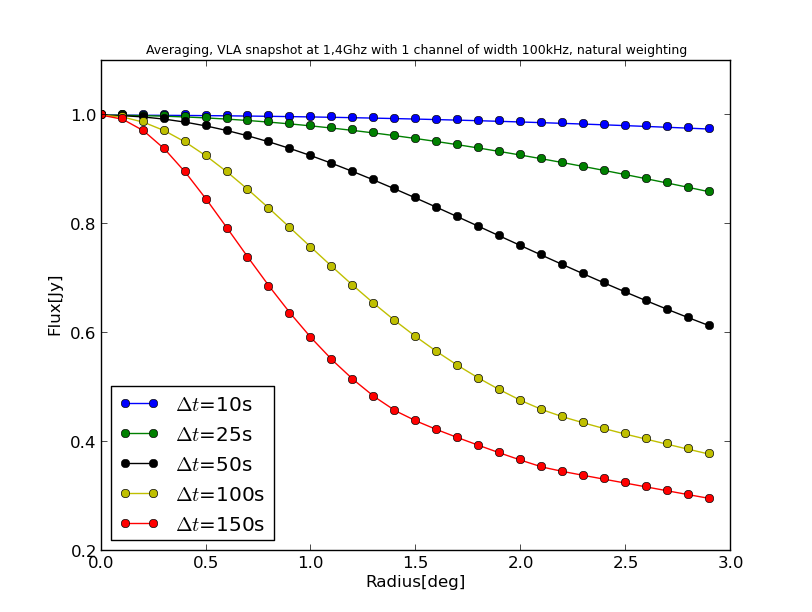
\includegraphics[width=1\textwidth]{./Figures/effect_time_averaging.png}\caption{The fall of the 
intensity of a 1Jy source move from the phase centre for $\Delta t$ integration synthesis at 100KHz 
bandwidth.}\label{timessear1}\end{minipage}
\begin{minipage}{0.38\linewidth}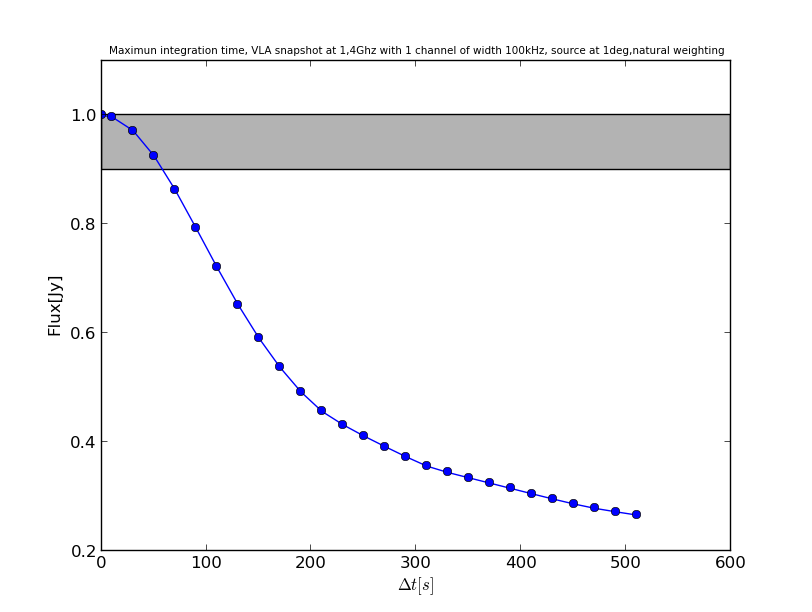
\includegraphics[width=1\textwidth]{./Figures/maximun_integration.png}\caption{(b)Response to a 1Jy 
source at 1deg, as a function of $\Delta t$ with 100KHz bandwidth}\label{timessear11}\end{minipage}\\
\begin{minipage}{0.38\linewidth}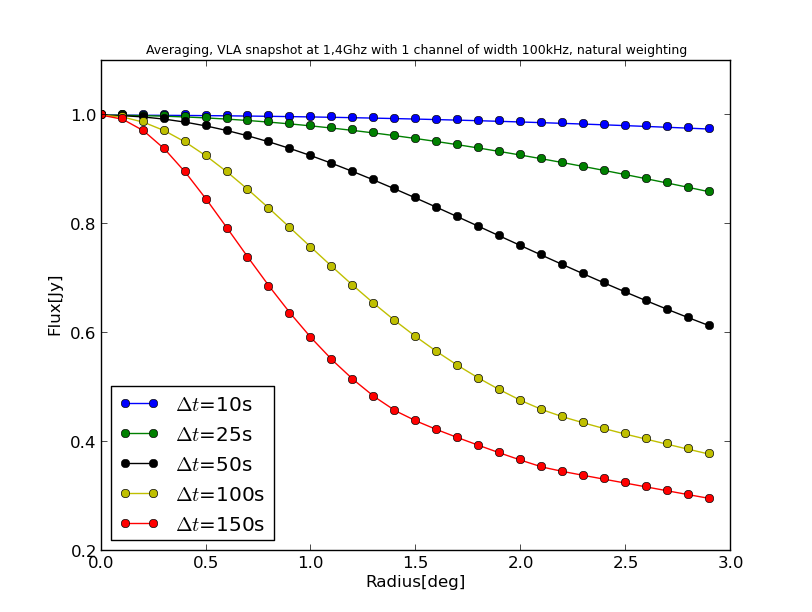
\includegraphics[width=1\textwidth]{./Figures/effect_time_averaging.png}\caption{The fall of the 
intensity of a 1Jy source move from the phase centre for $\Delta t$ integration synthesis at 100KHz 
bandwidth.}\label{timessear2}\end{minipage}
\begin{minipage}{0.38\linewidth}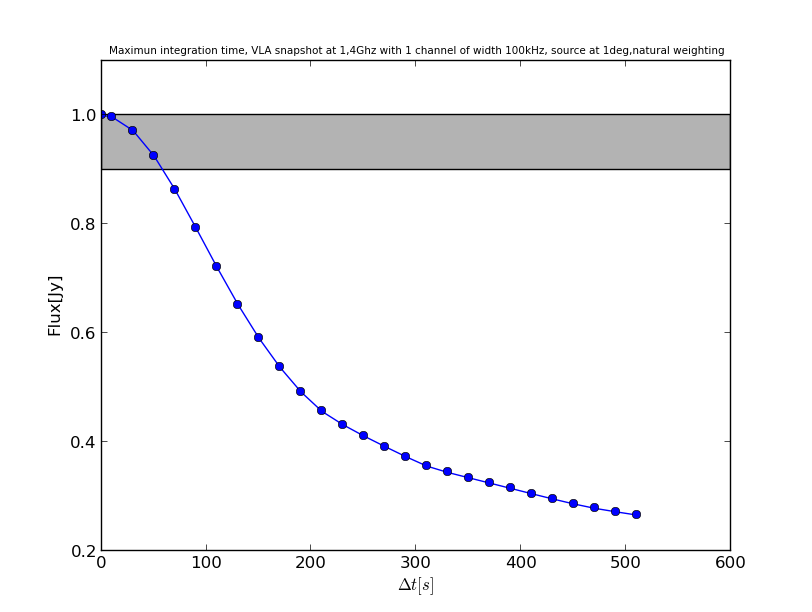
\includegraphics[width=1\textwidth]{./Figures/maximun_integration.png}\caption{The fall of the 
intensity of a 1Jy source move from the phase centre for $\Delta t$ integration synthesis at 100KHz 
bandwidth.}\label{fig:fig_5}\end{minipage}
\end{figure*}
Fortunately, since the response is maximal only for sources at the phase centre, an interesting approach is achieved by convolving the 
observed visibility with a  windowing function that depends on $(u,v)$ coordinates spacing (baseline dependent windowing function). 
However, a windowing function with a wide dynamic range spectrum is preferable in this work.
\subsection{Imaging}
From the full sky Radio Interferometry Measurement Equation (RIME) formalism (see Hamaka et \textit{al}, O.M. Smirnov (2010a)), in this 
case, the sampled visibilities can be presented mathematically as a $4\times n_t\times n_{\nu}$ matrix of four polarizations time and 
frequency dependent matrices each of size $n_t\times n_{\nu}$.
\begin{eqnarray*}
\mathbf{V}_{pq,(t,\nu)}^{samp}&=&\mathcal{\textbf{S}}_{pq,(t,\nu)}\cdot\mathbf{V}_{pq,(t,\nu)}\\
			      &=&\Bigg(\mathbf{V}_{pq,(t,\nu)}^{0},\mathbf { V } 
^1_{pq,(t,\nu)},\mathbf{V}^2_{pq,(t,\nu)},\mathbf{V}_{pq,(t,\nu)}^{3 } \Bigg)^T. \label{eqx:conv}
\end{eqnarray*}
Now, consider that $\mathcal{\textbf{W}}_{pq,(t,\nu)}$ is a $n_t \times n_{\nu}$ matrix that contained the weights of the baseline $(p,q)$ 
visibilities points. The weights of this matrix are given by a baseline dependent windowing function that we described in section 
\ref{baseline1} and section \ref{baseline2}.
The convolution operator is linear, therefore we can rewrite Eq.\ref{f4} in terms of a series of linear transformations as follow:
\begin{equation}
V_{pq}^{avg}= \mathbf{W}_{pq,(t,\nu)}^{block}\cdot 
\mathbf{S}_{pq,(t,\nu)}\cdot\mathbf{V}_{pq,(t,\nu)}.\label{eqbb:linear}
\end{equation}
Here, $\mathbf{W}_{pq,(t,\nu)}^{block}$ is a block diagonal matrix of size $(4n_t n_{\nu})\times(4n_t n_{\nu})$ and the 
block elements are $\mathbf{C}_{pq,(t,\nu)}\cdot\mathcal{\textbf{W}}_{pq,(t,\nu)}$ of size $n_t\times n_{\nu}$, where 
$\mathbf{C}_{pq,(t,\nu)}$ is the centre time interval and centre frequency interval sampling matrix of size $n_t\times n_{\nu}$. This
is the result of the time and frequency integration for the baseline $(p,q)$.

For a synthesis, the baseline $(p,q)$ made a full coverage in the $(u,v)$ plane. Therefore, we can  
package into a single matrix, $\mathbf{V}_{pq,}^{avg}$ of size $(4N_t N_{\nu})\times (4N_t N_{\nu})$ the 
weighted average visibilities of the  baseline $(p,q)$ during the synthesis as follows: 
\begin{equation}
\mathbf{V}_{pq}^{avg}= \mathbf{W}_{pq,(t,\nu)}^{block,n}\cdot\mathbf{S}_{pq,(t,\nu)}^{n}\cdot\mathbf{V}_{pq,(t,\nu)},\label{eq2:block}
\end{equation}
where $N_t$ and  $N_{\nu}$ are the number of time sample and frequency channels entering the Fourier domain. If the synthesis time is $T$ 
and the frequency range is $F$, then $T=N_t \times \Delta t$ and $F=N_{\nu}\times\Delta \nu$. The the size of 
$\mathbf{V}_{pq}^{avg}$ can also be written as $(4N_v^{pq})\times (4N_v^{pq})$, where $N_v^{pq}$ is the 
number of time and frequency visibilities for the baseline $(p,q)$). The matrix $\mathbf{W}_{pq,(t,\nu)}^{block,n}$ is a diagonal block 
matrix of size $(4N_v^{pq}n_t n_{\nu})\times (4N_v^{pq}n_t n_{\nu})$ where each diagonal block is the block diagonal matrix 
$\mathbf{W}_{pq,(t,\nu)}^{block}$ defined above and $n$ is the number of $\mathbf{W}_{pq,(t,\nu)}^{block}$. The sampled visibilities
$\mathcal{\textbf{S}}_{pq,(t,\nu)}^{n}\cdot\mathbf{V}_{pq,(t,\nu)}=\textbf{V}_{pq,(t,\nu)}^{samp,n}$ is a one row matrix of size 
$(N_v^{pq}4 n_t n_{\nu})\times (4 n_t n_{\nu})$ made of $\textbf{V}_{pq,(t,\nu)}^{samp}$ on top of each other. 
\begin{equation}
\mathbf{V}_{pq}^{avg}= \mathbf{W}_{pq,(t,\nu)}^{block,n}\cdot 
\mathbf{S}_{pq,(t,\nu)}^{n}\mathbf{F}\cdot\mathcal{I}_{l,m}^{sky},\label{eqv:linear}
\end{equation}
if the number of pixel in the sky model is $N_{pix}$, then the true sky image vector $\mathcal{I}_{l,m}^{sky}$ has a size of $4N_{pix}$ and 
$\textbf{F}$ is the Fourier transform operator of size $(4N_{pix})\times(4N_{pix})$. 

We are generally interested in using the total set of visibilities over baselines, time and frequencies, having $4\times N_v$ visibilities 
measured over all baselines  and $N_v=n_{bl}\times N_v^{pq}$ in this case. Here, $n_{bl}$ is the number of baseline. We can write
\begin{equation}
 \mathbf{V}_{all}^{avg}=\mathbf{A}\cdot\mathcal{I}_{l,m}^{sky}.
\end{equation}
Here, $\mathbf{A}$ is a matrix of size $(4N_v)\times (4N_{pix})$ made of 
$\mathbf{W}_{pq,(t,\nu)}^{block,n}\cdot\mathcal{S}_{pq,(t,\nu)}^{n}\cdot\mathbf{F}$ on top of each other. The 
dirty image, $\mathcal{I}_{l,m}^{D}$ of size $4N_{pix}$ can then be derived
\begin{equation}
\mathcal{I}_{l,m}^{D}=\mathbf{F}^{H}\cdot\mathbf{A}\cdot\mathcal{I}_{l,m}^{sky}.
\end{equation}
Here, $H$ represents the the conjugate transpose operation also known as a Hermitian transpose and $\mathbf{F}^{H}$ is the inverse 
Fourier transform operator of size $(4N_{pix})\times(4N_{pix})$.
% \begin{figure}
%   \subfloat[]{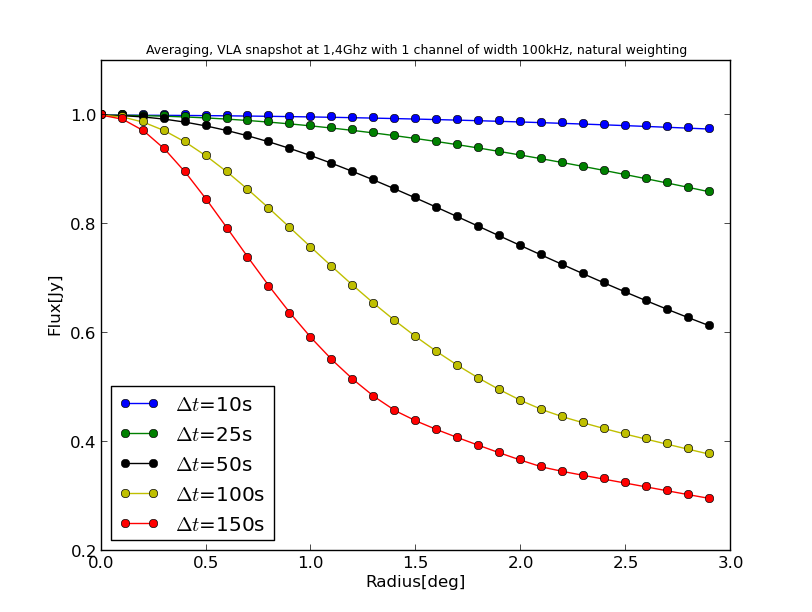
\includegraphics[width=0.18\textwidth, height=0.18\textwidth]{./Figures/effect_time_averaging.png}} 
%   \qquad
%   \subfloat[]{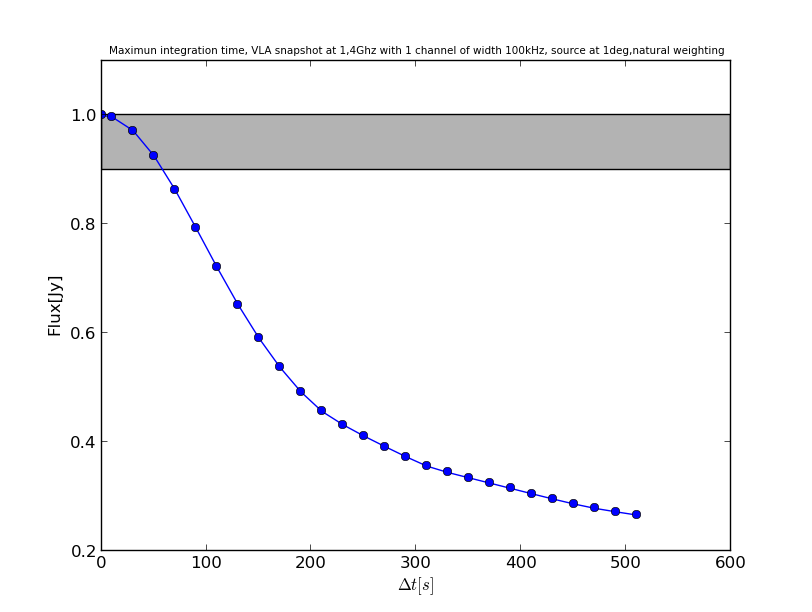
\includegraphics[width=0.18\textwidth,height=0.18\textwidth]{./Figures/maximun_integration.png}}
%   \qquad
%   \subfloat[]{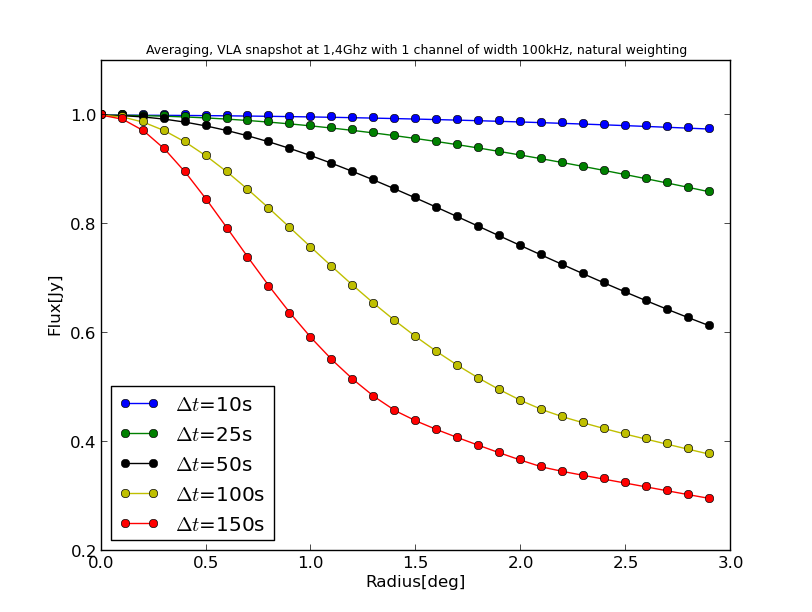
\includegraphics[width=0.18\textwidth, height=0.18\textwidth]{./Figures/effect_time_averaging.png}} 
%   \qquad
%   \subfloat[]{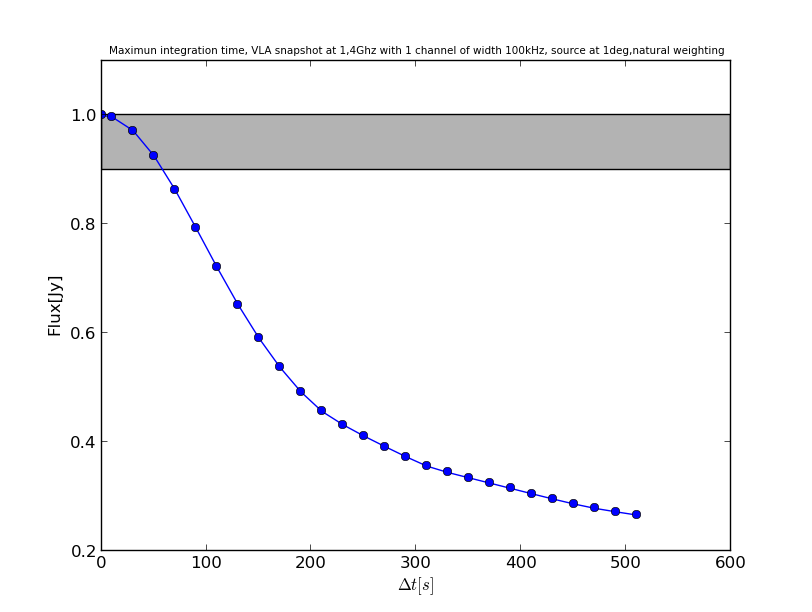
\includegraphics[width=0.18\textwidth,height=0.18\textwidth]{./Figures/maximun_integration.png}}
%   \caption{(a) The fall of the intensity of a 1Jy source move from the phase centre for $\Delta t$ integration synthesis at 100KHz 
% bandwidth. (b)Response to a 1Jy source at 1deg, as a function of $\Delta t$ with 100KHz bandwidth.}
% \end{figure}
\section{Data compression algorithm}
\label{baseline1}
\subsection{Description}
Missing spaces between sampled $(u,v)$ coordinates has huge dependences on the baseline length. However, the spacing between longer 
baselines $(u,v)$ coordinates are wider then the one on shorter baselines: this explained while sources are more distorted on longer 
baselines. We aims in this section, to describe the algorithm we use with a baseline-dependent windowing function to assign a proper 
weight to a data reference by a $(u,v)$ coordinate considering the \textit{spacing}\footnote{The \textit{distance} has also huge 
dependences on the baseline length and allow us to formally define the data
weight of a $uv$ point over the entire $uv$ plane.} between the baseline $(u,v)$ coordinates.

Fig.\ref{fig:uvcov} shows a snapshot coverage of an integration interval. For shorter baselines, the tracks are closer to the centre of 
rotation and for longer baselines the tracks are farther away from this centre. The \textit{dot marks} are the data for a sampled $(u,v)$ 
data, and the  arrows indicates the separation between $(u,v)$ coordinates and the centre $(u,v)$ coordinate. It is trivial to see on this 
figure that these separations are wider on longer baselines. The results of averaging is assigned to the centre $(u,v)$ coordinate coloured 
in red. 
\subsection{Methods}
In this section, we present the data compression algorithm we use to describe the weight of each sampled visibility during the 
integration time interval and and frequency interval. Now, let package the $(u,v)$ coordinates changes of a baseline $pq$ into a single 
matrix of size $n_t \times 2$.
\begin{equation}
\mathbf{U}_{pq,t}= \Bigg(\mathbf{u}_{pq,t_s}, \dots , \mathbf{u}_{pq,t_c}, \dots, \mathbf{u}_{pq,t_e}\Bigg)^T,
\end{equation}
where the indexes $s$, $c$ and $e$ references the integration interval starting, centre, and ending time respectively. The 
elements of $\mathbf{U}_{pq,t}$ are functions of time and frequency representing a $(u,v)$ coordinate. The frequency changes of the 
baseline coordinates can be package into a single vector of dimension $n_{\nu}$ 
\begin{eqnarray*}
 \mbox{\boldmath $\nu$}&=&\Bigg(\nu_s,\dots,\nu_c,\dots,\nu_e\Bigg)^T
\end{eqnarray*}
We define a norm, $||\cdot||_{m}$ on a $n_t \times 2$ matrix as follow:
\begin{eqnarray}
||\textbf{U}_{pq,t}||_{m}=\Bigg(||\mathbf{u}_{pq,t_s}||, \dots , ||\mathbf{u}_{pq,t_c}||, \dots, ||\mathbf{u}_{pq,t_e}||\Bigg),
\end{eqnarray}
where $||.||$ is the Euclidean norm.
\begin{definition}[Time direction spacing]
\label{def:1}
The matrix that model the spacing between the $(u,v)$ coordinates and the centre $(u,v)$ coordinate of a baseline $(p,q)$ across the time 
direction is defined as
\begin{eqnarray*}
 \mathbf{U}_{pq,t}^{s} &=&\frac{\nu_c}{c}\cdot\Bigg\{\mathbf{U}_{pq,t}-\mathbf{H}_{pq,t} \Bigg \},
\end{eqnarray*}
where $c$ is the speed of the light and $\mathbf{H}_{pq}$ is a matrix of size $n_t \times 2$ that model the centre $uv$-coordinate,
$\mathbf{H}_{pq,t}= \big(\mathbf{u}_{pq,t_c}, \dots , \mathbf{u}_{pq,t_c}, \dots, \mathbf{u}_{pq,t_c}\big)^T$.
\end{definition}
\begin{definition}[Frequency direction spacing]
\label{def:2}
The vector of size $n_{\nu}$ that model the spacing between the $(u,v)$ coordinates and the centre $(u,v)$ coordinate of a baseline $(p,q)$ 
across the frequency direction is defined as
\begin{eqnarray*}
\mathbf{d}^{T}_{\nu} &=&\frac{||\textbf{u}_{pq,t_c}||}{c}\cdot\Bigg\{\mbox{\boldmath 
$\nu$}-\nu_c\cdot\mathbf{g}^T_{\nu} \Bigg \},
\end{eqnarray*}
where  $\textbf{g}$ is a $1\times n_{\nu}$ unity matrix.
\end{definition}
\begin{definition}[Baseline dependent windowing function]
\label{def:3}
If $f_{pq}$ is a \textit{baseline dependent windowing function}, then:
\begin{eqnarray*}
 f_{pq}: \{\mathbf{\mathcal{R}},\mathbf{\mathcal{R}}\} &\rightarrow& \mathbf{\mathcal{R}}\\
                   d_{t_i},d_{\nu_j} &\mapsto& \frac{w_{t_i,\nu_j}}{\sum_{i=1}^{n_t}\sum_{j=1}^{n_{\nu}}w_{t_i,\nu_j}}.
\end{eqnarray*}
where $d_{t_i}$ is an element of the vector $\mathbf{d}_{t}=||\mathbf{U}_{pq,t}^{s}||_{m}$ and $d_{\nu_j}$ is an element of the vector 
$\mathbf{d}^{T}_{\nu}$.
\end{definition}
% where $\mathbf{x}_{pq}(t-t_c)=\bigg(\Big|\Big|\Big(u_{pq}'(t_s),v_{pq}'(t_s)\Big)\Big|\Big|,\dots, 
% \Big|\Big|\Big(u_{pq}'(t_e),v_{pq}'(t_e)\Big)\Big|\Big| \bigg)$ and 
% $\mathbf{y}_{pq}(\nu-\nu_c)=\bigg(\Big|\Big|\Big(u_{pq}''(\nu_s),v_{pq}''(\nu_s)\Big)\Big|\Big|,\dots, 
% \Big|\Big|\Big(u_{pq}''(\nu_e),v_{pq}''(\nu_e)\Big)\Big|\Big| \bigg)  $
% $1.)$ In Figures (\ref{fig1}) and (\ref{fig2}) we represented the ratio $\frac{\sigma_{meas,pq}}{\sigma_{av,pq}}$ as a function 
% of $\sum_{i}^{n} u_i((t_c-t_i)/\lambda))$ ($\sigma_{meas,pq},\sigma_{av,pq}$ are the per baselines CWF and averaging rms noise  
% respectively). We could also represented it as a function of baseline length. But, a uv-track corresponding to baseline aligned along the 
% Est-West direction has longer tracts compare to one aligned along the South-Nordth for the same integration and frequency band. Therefore,  
% $\frac{\sigma_{meas,pq}}{\sigma_{av,pq}}$ $v/s$ baselines length is ambiguous. We consider five baselines dependent 
% windowing sinc function, $Bl$-$sinc$ $wk$ (with an extended width of $(k-1)n$ time intervals and/or frequency channels and $k \geq 1$). The 
% experiment is done for two cases, figure (\ref{fig1}) is the one for $Bl$-$sinc$ $wk$ over both time-frequency and figure (\ref{fig2}) over 
% time. These figures shows that, the noise increases with baselines length.\\
% \begin{figure}
%   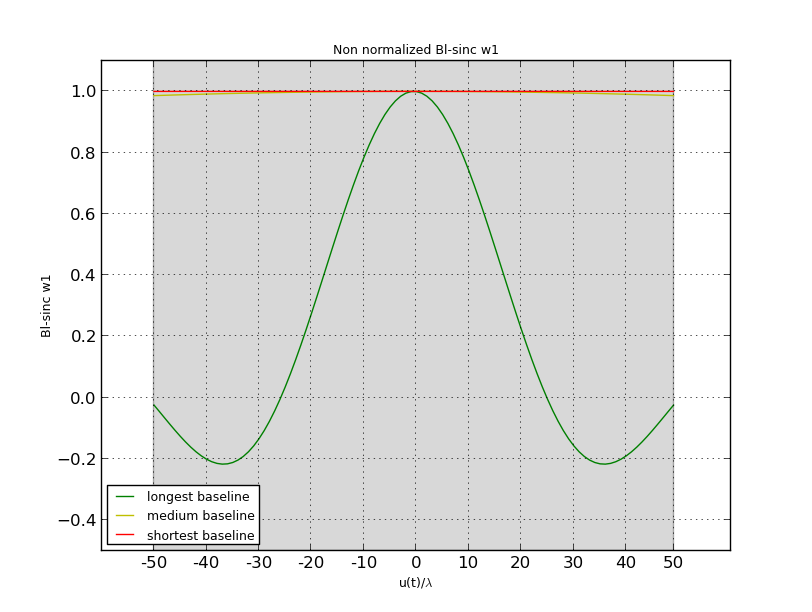
\includegraphics[width=0.4\textwidth, height=0.4\textwidth]{./Figures/longshortmid.png}
%   \caption{Snapshot coverage} \label{uvcov}
% \end{figure}
% \begin{figure}
%   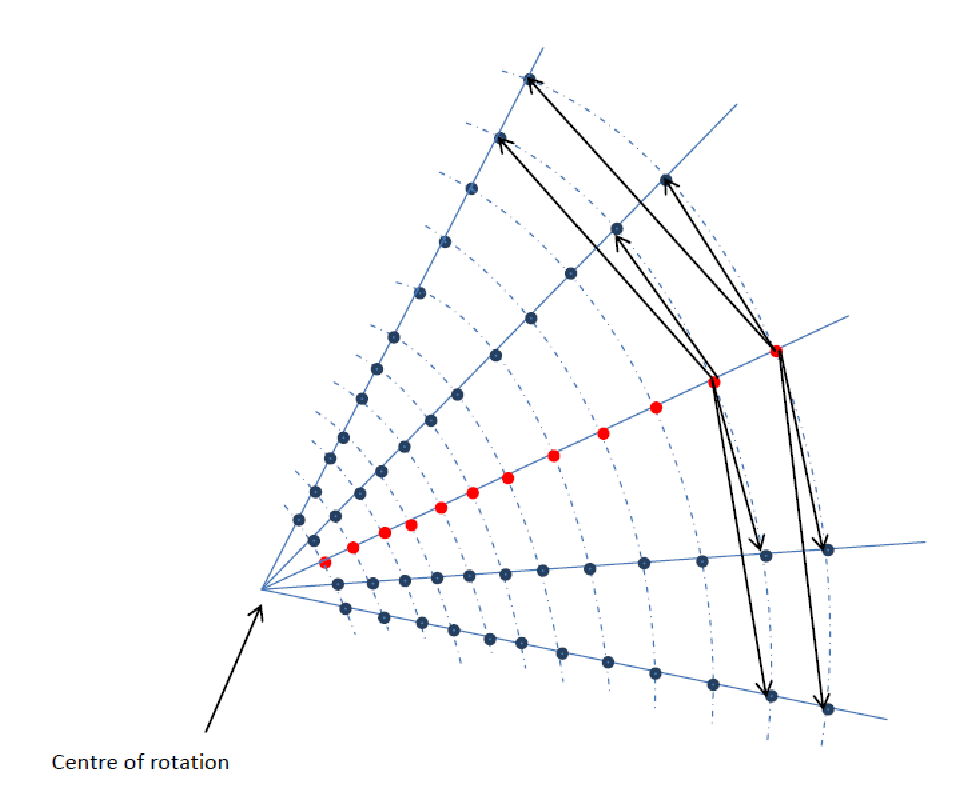
\includegraphics[width=0.4\textwidth, height=0.4\textwidth]{./Figures/uvcov.png}
%   \caption{Snapshot coverage} \label{uvcov}
% \end{figure}
\begin{figure*}
 \centering
\begin{minipage}{0.38\linewidth}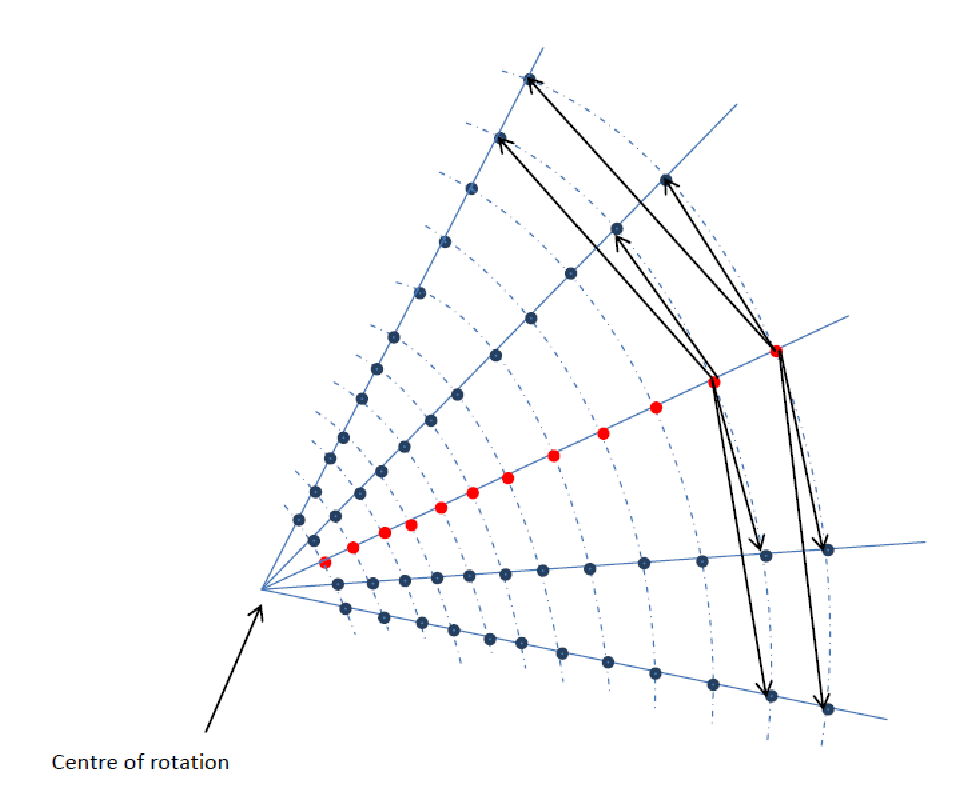
\includegraphics[width=1\textwidth]{./Figures/uvcov.png}\caption{Snapshot coverage}\label{fig:uvcov} 
\end{minipage}
\begin{minipage}{0.38\linewidth}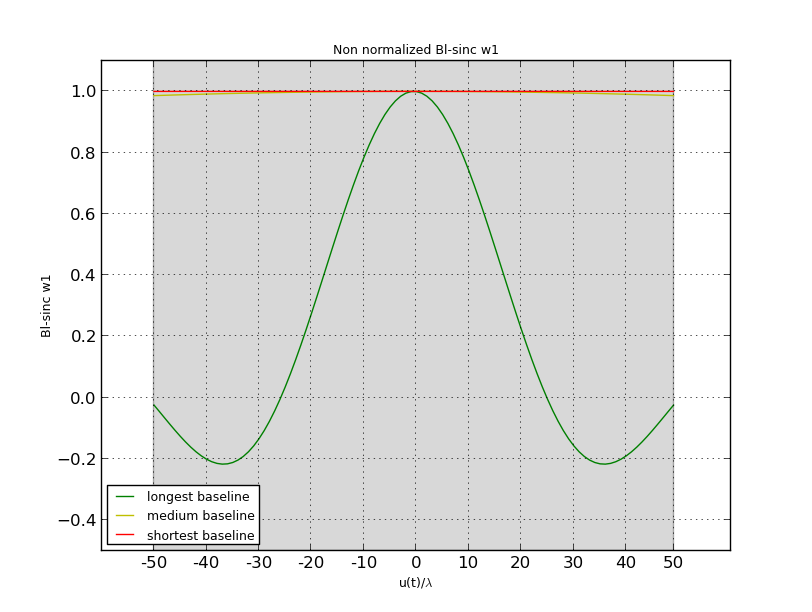
\includegraphics[width=1\textwidth]{./Figures/longshortmid.png}\caption{$Bl$-$sinc w1$ used to convolve the 
visibility data obtained from the long, medium and short baseline}\label{fig:fig_2b}
\end{minipage}
\end{figure*}
% \subsection{Cross-correlation with \textit{BDWF}}
% Taking a step back to eq \ref{}
% \begin{eqnarray*}
%  V^{meas}_{pq}(\mathbf{u}(t)/\lambda) &=&\sum_{t}\sum_{\nu} f_{pq}(\mathbf{d}_{t},\mathbf{d}_{\nu})\cdot 
% \mathbf{V}_{pq}^{obs}(t,\nu)\\
% 					  &=& \sum_{t}\sum_{\nu}\mathbf{W}_{pq}(t-t_c, \nu-\nu_c)\cdot \mathbf{V}_{pq}^{obs}(t,\nu)\\
% \end{eqnarray*}
\subsection{Noise  analysis}
% In this section, theoretical expressions of the noise of correlator windowing functions (CWF) are derived. 
% Simulations results shows that when the overlap width of CWF is increased, the noise in the sky map is reduced. Furthermore, 
% the noise reduces more rapidly when the overlap is done over both time intervals and frequency channels. For convenience, we have 
% chosen to derive the analytical expression for the noise of a CWF at the phase centre. For the analysis we used a simulated 
% VLA, 1min30s synthesis, with a 1,5s integration time at 1,4Ghz, with 100 channels of width 1kHz. We fill this simulated measurement set 
% with 1Jy thermal noise and we used a sinc as a CWF.
For convenience, in this section, we  analyse the centre pixel noise of a sky map after we had apply a baseline dependent windowing 
function during the time and frequency integration. The brightness of the 
naturally weighted central pixel is estimate by (see the inverse Fourier transform of equation (19-2) in 
\cite{1} ).
\begin{eqnarray*}
\widetilde{\mathcal{I}}(0,0)&=&\frac{1}{N_{v}}   \sum_{k=1}^{N_{v}} V_{all,k}^{avg}\\
	          &=&\frac{1}{N_{v}}   \sum_{pq,k=1}^{N_{v}^{pq}} V_{pq,k}^{avg}\\
	          &=&\frac{1}{N_{v}}   \sum_{pq,k=1}^{N_{v}^{pq}}\Big(\sum_{i=1}^{n_t}\sum_{j=1}^{n_{\nu}} 
f_{pq,(dt_i,d\nu_j)}V_{pq,(t_i,\nu_j)}^{samp}\Big).
\end{eqnarray*}
Here, the variable $k$ run through the baseline $(p,q)$ timeslots. The  overall rms noise is given by
\begin{eqnarray*}
\sigma^2	&=& 
\frac{\sigma^{2}_{samp} }{N_{v}^{2}}\Big(\sum_{pq,k=1}^{N_{v}^{pq}}\sum_{i=1}^{n_t}\sum_{j=1}^{n_{\nu}}f_{pq,(dt_i,d\nu_j)}^{2}\Big) 
,\label{Equ:BDWnoise}
\end{eqnarray*}
where  $\sigma_{samp}$ is the per sampled visibility noise
% Where $W^{pq}$ is a normalized CWF; $\lambda$, $t_c$ are the observed wavelength and centre of the integration 
% respectively. $N_{meas}$ is the number of the measured visibilities. The observed visibilities of baseline $pq$  are 
% $V^{pq}_{obs}(u(t/\lambda))$, $n$ is the number of time intervals  and/or frequency channels within the within the width of the CWF.
% %and defined as % and is given by
% let introduced jjjjjjjjjjjjjjs  sjjs lkk xxxxxxxxxxxx xxxxxxxxxxxx xxxxxxxxxx xxxxxxxxxx xxx ,xssss, s,,,sssssx, xxxxxxxxxx,x 
% xxxxxxxxxxxxxx,,xxxxxxxxxxxx, write more here to explain
% \begin{eqnarray**}
% \widetilde{I}(0,0)&=&\frac{1}{N_{meas}}   \sum_{all-pq}\Big(\sum_{t}\sum_{\nu}f_{pq}(\mathbf{d}_{t},\mathbf{d}_{\nu})\cdot 
% \mathbf{V}_{pq}^{obs}(t,\nu)\Big)
% \end{eqnarray**}
% \begin{eqnarray*}
% 		\sigma_{meas, pq}^2	&=&var\Big(\sum_{t}\sum_{\nu}f_{pq}(\mathbf{d}_{t},\mathbf{d}_{\nu})\cdot 
% \mathbf{V}_{pq}^{obs}(t,\nu)   
% \Big)\\
% 		&=&\sum_{t}\sum_{\nu}f_{pq}^{2}(\mathbf{d}_{t},\mathbf{d}_{\nu}) \sigma_{obs}^2 
% \end{eqnarray*}
% where $\sigma_{obs}$ is the expected rms noise per observed visibility. By replacing eq \ref{1} into eq \ref{1} we obtained
% \begin{eqnarray*}		
% \sigma^2	
% &=&\Big(\frac{\sigma_{obs}}{N_{meas}}\Big)^2\cdot\sum_{all-pq}\Big(\sum_{t}\sum_{\nu}f_{pq}^{2}(\mathbf{d}_{t},\mathbf{d}_{\nu})\Big)
% \end{eqnarray*}
% If $f_{pq}$ is a boxcar function, then $\sigma^2 =\frac{1}{N_{meas} \times n_t \times n_{\nu}} \sigma_{obs}^2$ ,
% and can be expressed as a function of the number of the observed visibilities, $N_{obs}$ as $\sigma^2=\frac{1}{N_{obs}\times 
% n_{\nu}} \sigma_{obs}^2$.
% % \begin{eqnarray**}
% % \sigma^2	   &=&\frac{1}{N_{obs}\times n_{\nu}} \sigma_{obs}^2
% % \end{eqnarray**}
\section{Out FoV sources suppression algorithm}
\label{baseline2}
\subsection{Description}
In theory, windowing functions and signals generally extend to  infinity. Unfortunately, in practice, filtering a signal with a low pass 
filter, one need to define a cut-off interval. Therefore, if one  wants to achieve sufficiently an accurate  estimate of the 
windowing function ideal spectrum, one need a wide cut-off interval as far as the spectrum approaches the ideal when the windowing function 
order increases. An overlap baseline dependent windowing function aims to extend the order of the baseline dependent windowing function in 
such a way that, we approaches the ideal spectrum.
%, but by maintaining the same cut-off interval like the boxcar one. 
The only drawback of this technique is the increased of the time needed for processing the output sample of the signals being integrate.  
\subsection{Methods}
The weight of a visibility is not defined by a unique baseline dependent windowing, but by the strength of the correlation between the 
overall  overlapping baseline dependent windowing functions on the visibility. Now, consider that $f^{a}_{pq}$ is an overlap-\textit{BDWF} 
of width  $\Delta t$ and $\Delta \nu$ across the time and frequency direction respectively.
\begin{definition}[Baseline dependent windowing function]
\label{def:4}
if $\Delta_l t$ and $\Delta_l \nu$ are the overlap time interval and frequency interval of the baseline dependent windowing function  
$f_{pq}^{a_0}$ respectively  and $\Big\{f_{pq}^{a_1},f_{pq}^{a_2},f_{pq}^{a_3}, \dots \Big\}$ the set of \textit{BDWF} overlapping  on the 
\textit{left hand side} of $f_{pq}^{a_0}$ then the resulting \textit{BDWF} within $\Delta_l t$ and $\Delta_l \nu$ is defined as
\begin{eqnarray*}
 g^{lhs}_{pq}: \{\mathbf{\mathcal{R}},\mathbf{\mathcal{R}}\} &\rightarrow& \mathbf{\mathcal{R}}\\
                   d_{t_i},d_{\nu_j} &\mapsto& \frac{1}{N_{lhs}}\Bigg(\sum_{k}f_{pq,(d_{t_i},d_{\nu_j})}^{a_k} 
+ f_{pq,(d_{t_i},d_{\nu_j})}^{a_0}\Bigg).
\end{eqnarray*}
Here, $N_{lhs}$ is the normalization term defined as
\begin{eqnarray*}
N_{lhs}=\sum_{i=1}^{n_{lt}}\sum_{j=1}^{n_{l\nu}}\Bigg(\sum_{k}f_{pq,(d_{t_i},d_{\nu_j})}^{a_k} + f_{pq,(d_{t_i},d_{\nu_j})}^{a_0} \Bigg),
\end{eqnarray*}
where $n_{lt}$ and $n_{l\nu}$ are the number of $(u,v)$ coordinates changes and frequency changes  within $\Delta_l t$ and $\Delta_l \nu$ 
respectively.
\end{definition}
\begin{definition}[Baseline dependent windowing function]
 \label{def:4}
 if $\Delta_r t$ and $\Delta_r \nu$ are the overlap time and frequency interval of a \textit{BDWF} $f_{pq}^{a_0}$ 
respectively and  $\Big\{f_{pq}^{a_1},f_{pq}^{a_2},f_{pq}^{a_3}, \dots \Big\}$ the set of \textit{BDWF} overlapping on the \textit{right 
hand side} of $f_{pq}^{a_0}$, then the 
resulting \textit{BDWF} within $\Delta_r t$ and $\Delta_r \nu$ is defined as
\begin{eqnarray*}
 g^{rhs}_{pq}: \{\mathbf{\mathcal{R}},\mathbf{\mathcal{R}}\} &\rightarrow& \mathbf{\mathcal{R}}\\
                   d_{t_i},d_{\nu_j} &\mapsto& 
\frac{1}{N_{rhs}}\Bigg (f_{pq,(d_{t_i},d_{\nu_j})}^{a_0}+\sum_{k}f_{pq,(d_{t_i},d_{\nu_j})}^{a_k}\Bigg ).
\end{eqnarray*}
Here, $N_{rhs}$ is the normalization term defined as
\begin{eqnarray*}
N_{rhs}=\sum_{i=1}^{n_{rt}}\sum_{j=1}^{n_{r\nu}}\Bigg(f_{pq,(d_{t_i},d_{\nu_j})}^{a_0} + \sum_{k}f_{pq,(d_{t_i},d_{\nu_j})}^{a_k}\Bigg),
\end{eqnarray*}
where $n_{rt}$ and $n_{r\nu}$ are the number of $(u,v)$ coordinates changes and frequency changes  within $\Delta_r t$ and $\Delta_r \nu$ 
respectively.
\end{definition}
From the above definitions, the following derivation is trivial 
\begin{equation*}
 \Big\{\Delta t,\hspace{0.17cm}\Delta \nu \Big\}=\Big\{\Delta_l t \cup \Delta_u t \cup \Delta_r t, \hspace{0.17cm}\Delta_l \nu \cup 
\Delta_u \nu \cup \Delta_r \nu \Big\},
\end{equation*}
where $\Delta_u t$ and $\Delta_u \nu$ are $f_{pq}^{a_0}$ uncorrelated time  and frequency interval respectively. They follows the below 
rules 
\begin{eqnarray*}
 \Delta_u t= \left\{ 
  \begin{array}{l l}
     \cup\{t_i\}_{i=s',\hspace{0.1cm} s' \geq s+1}^{c', \hspace{0.1cm}c'\leq c-1} & \quad \text{if $n_{lt}+n_{rt}< n_t$}\\
      \{t_c\}& \quad \text{if $n_{lt}+n_{rt} = n_t$}\\
       \emptyset  & \quad \text{otherwise}
  \end{array} \right.
\end{eqnarray*}
\begin{eqnarray*}
 \Delta_u \nu= \left\{ 
  \begin{array}{l l}
     \cup\{\nu_i\}_{i=s',\hspace{0.1cm} s'\geq s+1}^{c', \hspace{0.1cm}c'\leq c-1} & \quad \text{if $n_{lt}+n_{rt} < n_t$}\\
      \{\nu_c\}& \quad \text{if $n_{lt}+n_{rt} = n_t$}\\
       \emptyset  & \quad \text{otherwise}
  \end{array} \right.
\end{eqnarray*}
The resulting \textit{BDWF} becomes $g_{pq}$ described as
\begin{eqnarray*}
g_{pq} = \left\{ 
  \begin{array}{l l}
    g^{lhs}_{pq} & \quad \text{if $(t,\nu) \in (\Delta_l t, \Delta_l \nu)$}\\
    f^{a_0}_{pq} & \quad \text{if $(t,\nu) \in (\Delta_u t, \Delta_u \nu)$}\\
    g^{rhs}_{pq}& \quad \text{if $(t,\nu) \in (\Delta_r t, \Delta_r \nu)$}
  \end{array} \right.
\end{eqnarray*}
\subsection{Noise analysis}
The  overall rms noise is given by
\begin{eqnarray*}
\sigma^2	&=& 
\frac{\sigma^{2}_{samp} }{N_{v}^{2}}\Big(\sum_{pq,k=1}^{N_{v}^{pq}}\sum_{i=1}^{n_t}\sum_{j=1}^{n_{\nu}}g_{pq,(dt_i,d\nu_j)}^{2}\Big) 
,\label{Equ:OBDWnoise}
\end{eqnarray*}
\subsection{Windowing functions}
In signal processing a windowing function is a mathematical function that is zero-values outside of some chosen interval, and when another 
function or a signal is multiplied by the windowing function, the product is also zero-values outside the interval.
In this section, we evaluation the Peak Sidelobe Level (PSL), the Main 
Lobe width (MLW) and the Sidelobes Roll-off (SLR) of some windowing functions spectrum. This study will allow us to make 
a suitable choice of the window that by tapering with the sky, we conserve the brightness of sources in the field of 
interest and attenuate sidelobes confusion from strong sources out of the field of interest.
\subsubsection{Boxcar window: natural weighting}
This windowing function take a hunk of the data without modification, and  this leads to discontinuities at the edges\footnote{unless it 
happens that the signal  fit exactly with the windowing function width. Nevertheless, it is rare to find such a situation.}. For 
a cut-off frequency interval  $[-\nu_a,\nu_a]$ the boxcar windowing function is defined as:
\begin{equation}
\Pi_{u}=\left\{
\begin{array}{rl}
1 & \mbox{$-\nu_a \leq \nu \leq \nu_a$} \\
0 & \mbox{otherwise}
\end{array}\right.
\end{equation}
%and it Fourier transform is $\mathcal{F}^{-1}\big\{\Pi_{u}\big\}=sinc\big(\pi ||u(t/\lambda_a)|| l\big)$.\\
Fig.\ref{fig:fig_box} and Fig.\ref{fig:fig_box_freq} gives the graph of $\Pi_{u}$ and its spectrum respectively. The blue and 
the red curve of Fig.\ref{fig:fig_box_freq} are the spectrum of $\Pi_{u}$ for a frequency cut-off interval, $[-\nu_a,\nu_a]$ and 
$[-\nu_a/2,\nu_a/2]$ respectively. We noticed that when the cut-off interval is large, the MLW of the spectrum is 
narrower, the PSL is lower and the SLR drop faster. 
% The main lobe 
% extends from $-1/(2\nu_a)$ to $1/(2\nu_a)$, 
% beyond that the function oscillates at a constant rate while the amplitude gradually dies out. The larger the $\nu_a$, the narrower the 
% central peak and the oscillations.
\subsubsection{Gaussian window}
A Gaussian windowing function centred at mean zero with standard deviation, $\sigma$ can be described as 
\begin{equation}
  G_{u}= e^{-b\nu^{2}}.
\end{equation}
Here, $b=(2\sigma^2)^{-1}$ and  $\mathcal{F}^{-1}\big\{G_{u}\big\}=\sqrt{\frac{b}{\pi}}e^{-cl^2}$, where $c=\pi^2/b$.
This shows us that the inverse Fourier transform of a Gaussian with standard deviation $\sigma$ is a Gaussian with a standard 
deviation $\sigma '= (2\pi\sigma)^{-1}$. 

Fig.\ref{fig:fig_gauss} and Fig.\ref{fig:fig_gauss_freq} gives the graph of $G_{u}$ and its spectrum respectively, where $G_{u}$ 
is truncate within the cut-off frequency interval $[-\nu_a,\nu_a]$, with $b = 3$ for the blue curve and $b=5$ for the red one. We noticed 
that when the standard deviation is large, the MLW of the spectrum is narrower, the PSL is higher and the SLR drop slowly compare to a 
smaller standard deviation.
\subsubsection{Butterworth}
The frequency response of the Butterworth filter is flat  in the pass band, and rolls off towards zero in the stop band, and it is 
characterized by two independent parameters, the cut-off frequency 
$\nu_a$ and the order $p$. These two parameters controls the 
bandwidth and side lobes  attenuation. The frequency response of the Butterworth is given by 
\begin{equation}
B_u= \Big(1 + (\nu/\nu_a)^{2p}\Big)^{-1}.
\end{equation}
%Fig.\ref{fig:fig_butter} and Fig.\ref{fig:fig_butter_freq} gives the graph of $B_{u}$ and its spectrum respectively. 
For the same frequency interval $[-\nu_a,\nu_a]$, we plotted  three curves $\{p=1, p=3, p=5\}$ of $B_{u}$ in Fig.\ref{fig:fig_butter} and 
their corresponding spectrum in Fig.\ref{fig:fig_butter_freq}.  We noticed 
that when the other $p$ is getting bigger, the MLW of the spectrum is conserved, while the PSL is getting higher and the SLR is 
dropping  faster.
\subsubsection{First order prolate spheroidal wave function}
\subsubsection{Sinc window}
In theory, the sinc window  is an infinitely large convolution filter as it is non zero everywhere, and its inverse Fourier 
Transform produces
 the ideal filter kernel (the boxcar windowing function). The sinc is defined as follow:
\begin{equation}
S_u= sinc\big(\pi bu(t/\lambda_a)\big).
\end{equation}
However, in practice some one need to defined a cut-off interval where the window is considered to be non zero, and zero out of this 
cut-off interval. Fig.\ref{fig:fig_sinc} and Fig.\ref{fig:fig_sinc_freq} gives the graph of $S_{u}$ and its spectrum respectively, where 
$S_{u}$ is truncate within the cut-off frequency interval $[-\nu_a,\nu_a]$. We noticed that when the cut-off frequency interval is large 
(Fig.\ref{fig:fig_sinc_freq}, blue curve), the spectrum becomes perfectly flat at the passband while the MLW becomes narrower,  the PSL 
becomes lower and the SLR drop faster compare to a cut-off frequency of $[-\nu_a,\nu_a]$ (Fig.\ref{fig:fig_sinc_freq}, red curve). \\
\begin{tabular}{*3{c}}
 \multicolumn{3}{|c|}{}\\
 \begin{tabular}{|l|l|l|l|}
  \footnotesize Windows &\textbf{\footnotesize MLL (-3db)}&\textbf{\footnotesize PSL (db)} &\textbf{\footnotesize SLR (db/octave) }  \\
  \hline\hline
  {\footnotesize $\Pi_{u}$} &{\footnotesize $\approx 0,073$} &{\footnotesize $-6,68$}&{\footnotesize $-6,78$}\\
  {\footnotesize $\mathcal{F}^{-1}\{\Pi_{u}$\}} &{\footnotesize  $\approx0,306$}&{\footnotesize  $-11,22$}&{\footnotesize  $-12,42$} \\
  {\footnotesize $G_{u}$} & {\footnotesize $\approx0,0736$}&{\footnotesize  $-30,28$}&{\footnotesize  $-14,5$}\\ 
  {\footnotesize $B_{u}$} &{\footnotesize  $\approx0,079$} &{\footnotesize $-10,08$ }&{\footnotesize  $-15,39$}\\
  {\footnotesize $P_{u}$} &{\footnotesize  $\approx- $} &{\footnotesize $ -$ }&{\footnotesize  $ -$}
  \end{tabular}& \label{BDWBnoise}
\end{tabular}\\
A windowing function with a narrower main lobe width for a better spectral resolution, lower PSL to have less
masking of nearby sources, and faster SLR to have less masking for far away sources  is preferably in this work. 
Nevertheless, The energy is more concentrated in the frequency domain main lobe when the  lobe width is narrower. Therefore, the frequency 
domain of the boxcar  and the Butterworth window look similar, but the other of the Butterworth frequency domain can be control with the 
goal to concentrate more energy in the frequency main lobe. However, the  sinc window is preferable as we expect in this work, signals in a 
wide dynamic range.
\subsubsection{Noise  and comparison}
The methods described in section (\ref{baseline1}) and section (\ref{baseline2}) are use in this subsection to evaluate the 
theoretical noise, $f_{pq}$ and $g_{pq}$ are replaced in  Eq.\ref{Equ:BDWnoise} and 
Eq.\ref{Equ:OBDWnoise} respectively by the windowing functions described above. Table (\ref{BDWBnoise}) and 
(\ref{OBDWBnoise}) summarize the theoretical noise where these functions are used as a baseline dependent 
windowing and as an overlap baseline dependent windowing functions respectively. \\
\begin{tabular}{*3{c}}
 \multicolumn{3}{c}{}\\
  \hspace{-1.cm}\begin{tabular}{|c|c|}
  \textbf{$f_{pq}$}&\textbf{\footnotesize Theoretical noise} \\
  \hline\hline
  {\footnotesize $\Pi_{u}$} &{\footnotesize 1,066} \\ 
  {\footnotesize $\mathcal{F}^{-1}\{\Pi_{u}$\}} &{\footnotesize 1,066} \\ 
  {\footnotesize $G_{u}$} & {\footnotesize 1,334}\\ 
  {\footnotesize $B_{u}$} &{\footnotesize 1,066} \\
  {\footnotesize $\mathcal{F}^{-1}\{B_{u}$\}} &{\footnotesize 1,066} \\ 
  {\footnotesize $P_{u}$} & {\footnotesize 1,334}
  \end{tabular}& \label{BDWBnoise}
   \begin{tabular}{|c|c|}
  \textbf{$g_{pq}$}&\textbf{\footnotesize Theoretical noise} \\
  \hline\hline
  {\footnotesize $\Pi_{u}$} &{\footnotesize 1,066} \\ 
  {\footnotesize $\mathcal{F}^{-1}\{\Pi_{u}\}$} &{\footnotesize 1,066} \\
  {\footnotesize $G_{u}$} & {\footnotesize 1,334}\\ 
  {\footnotesize $B_{u}$} &{\footnotesize 1,066} \\
  {\footnotesize $\mathcal{F}^{-1}\{B_{u}$\}} &{\footnotesize 1,066} \\ 
  {\footnotesize $P_{u}$} & {\footnotesize 1,334}
  \end{tabular} \label{OBDWBnoise}
\end{tabular}
\\
\\
\\
\begin{figure*}
  \centering
  \begin{minipage}{0.36\linewidth}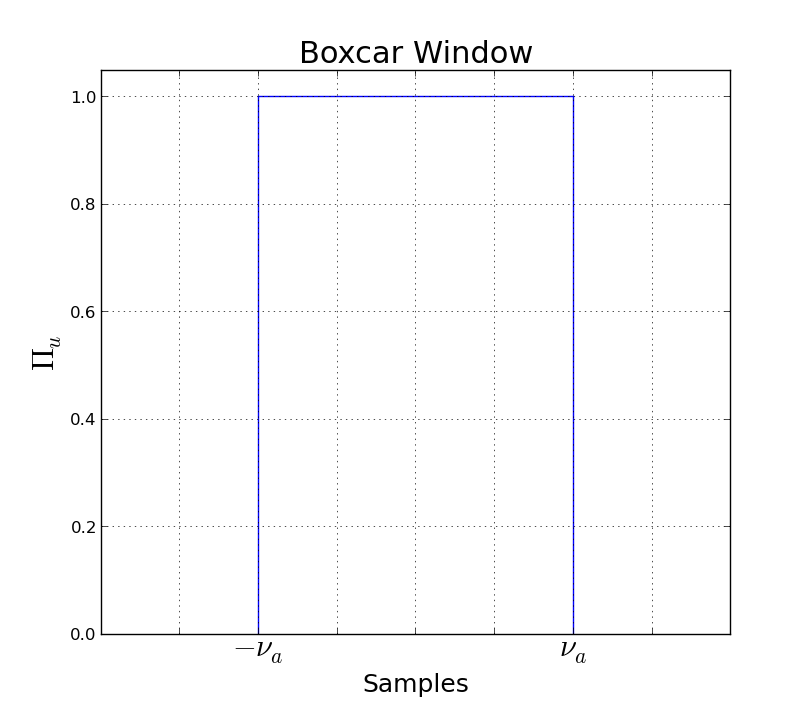
\includegraphics[width=1\textwidth]{./Figures/rect.png}\caption{Boxcar windowing 
function.}\label{fig:fig_box}\end{minipage}
\begin{minipage}{0.36\linewidth}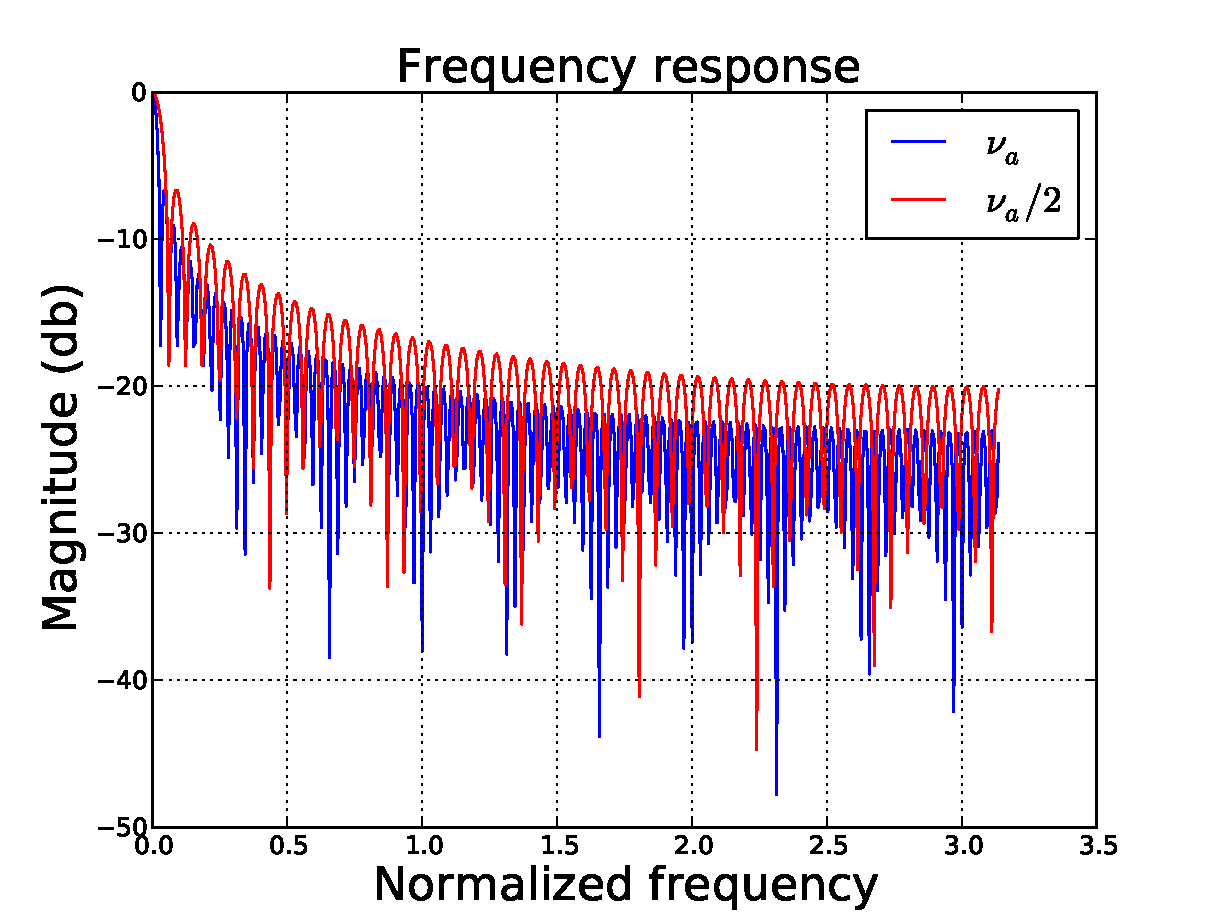
\includegraphics[width=1\textwidth]{./Figures/freq_resp_box.pdf}\caption{Overlap 
		\textit{BDWF's}: $\Delta_u t= [225, 250]$.}\label{fig:fig_box_freq}\end{minipage}\\
\begin{minipage}{0.36\linewidth}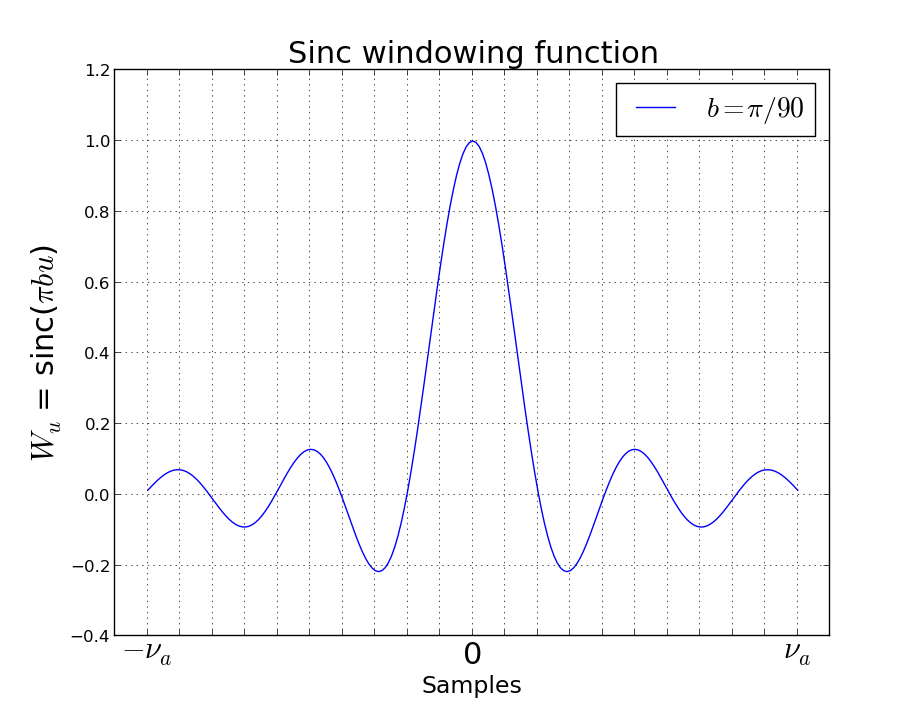
\includegraphics[width=1\textwidth]{./Figures/sinc.png}\caption{Overlap 
		\textit{BDWF's}: $\Delta_u t=\{250\}$.}\label{fig:fig_sinc}\end{minipage}
\begin{minipage}{0.36\linewidth}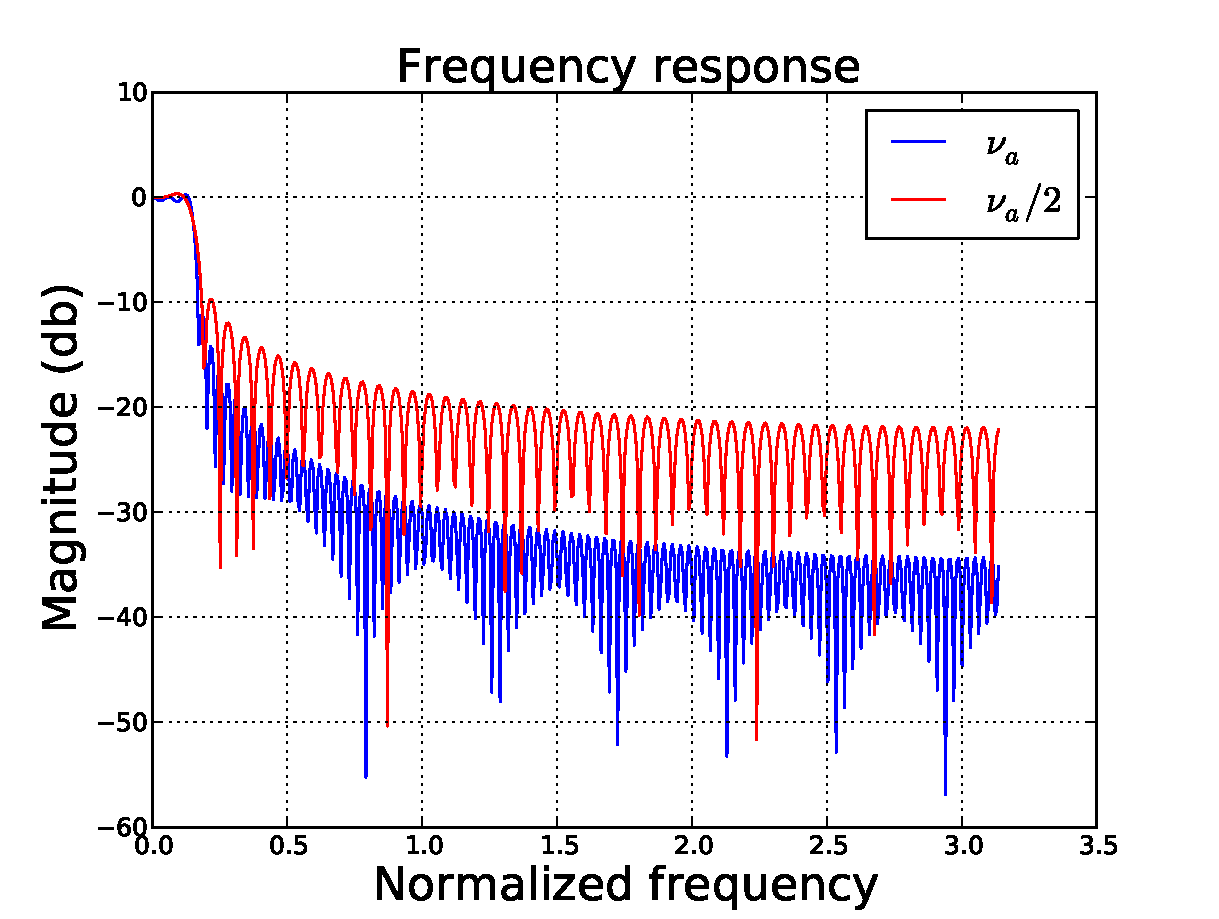
\includegraphics[width=1\textwidth]{./Figures/freq_resp_sinc.pdf}\caption{Overlap 
		\textit{BDWF's}: $\Delta_u t=\emptyset$.}\label{fig:fig_sinc_freq}\end{minipage}\\
\begin{minipage}{0.36\linewidth}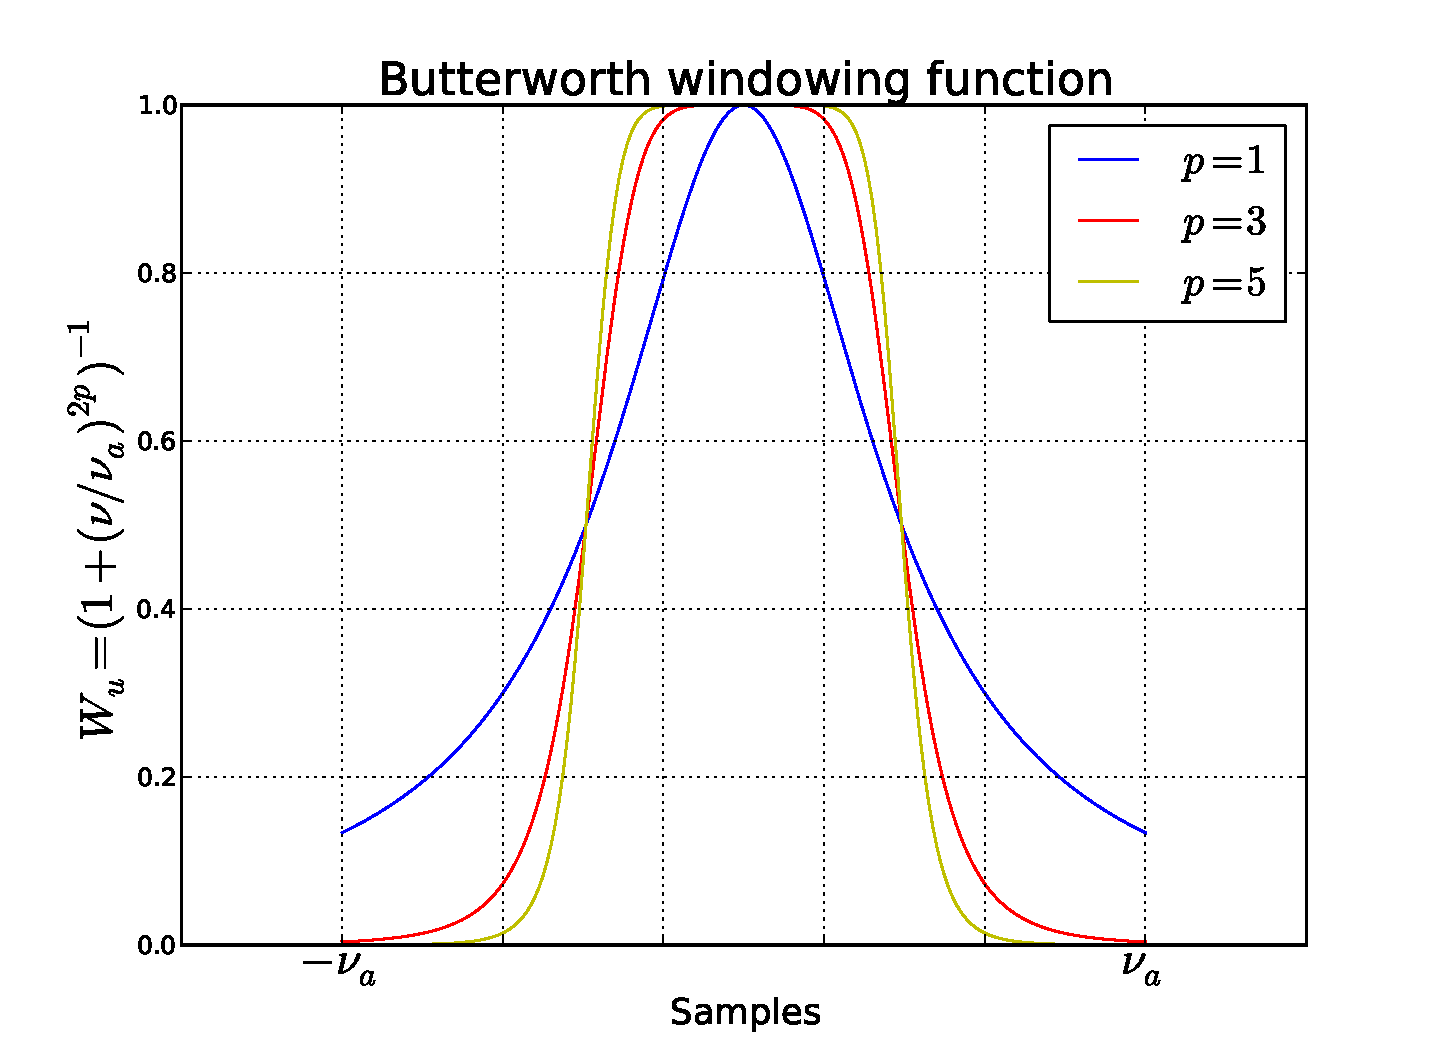
\includegraphics[width=1\textwidth]{./Figures/Butterwordth.pdf}\caption{Overlap 
		\textit{BDWF's}: $\Delta_u t=\{250\}$.}\label{fig:fig_butter}\end{minipage}
\begin{minipage}{0.36\linewidth}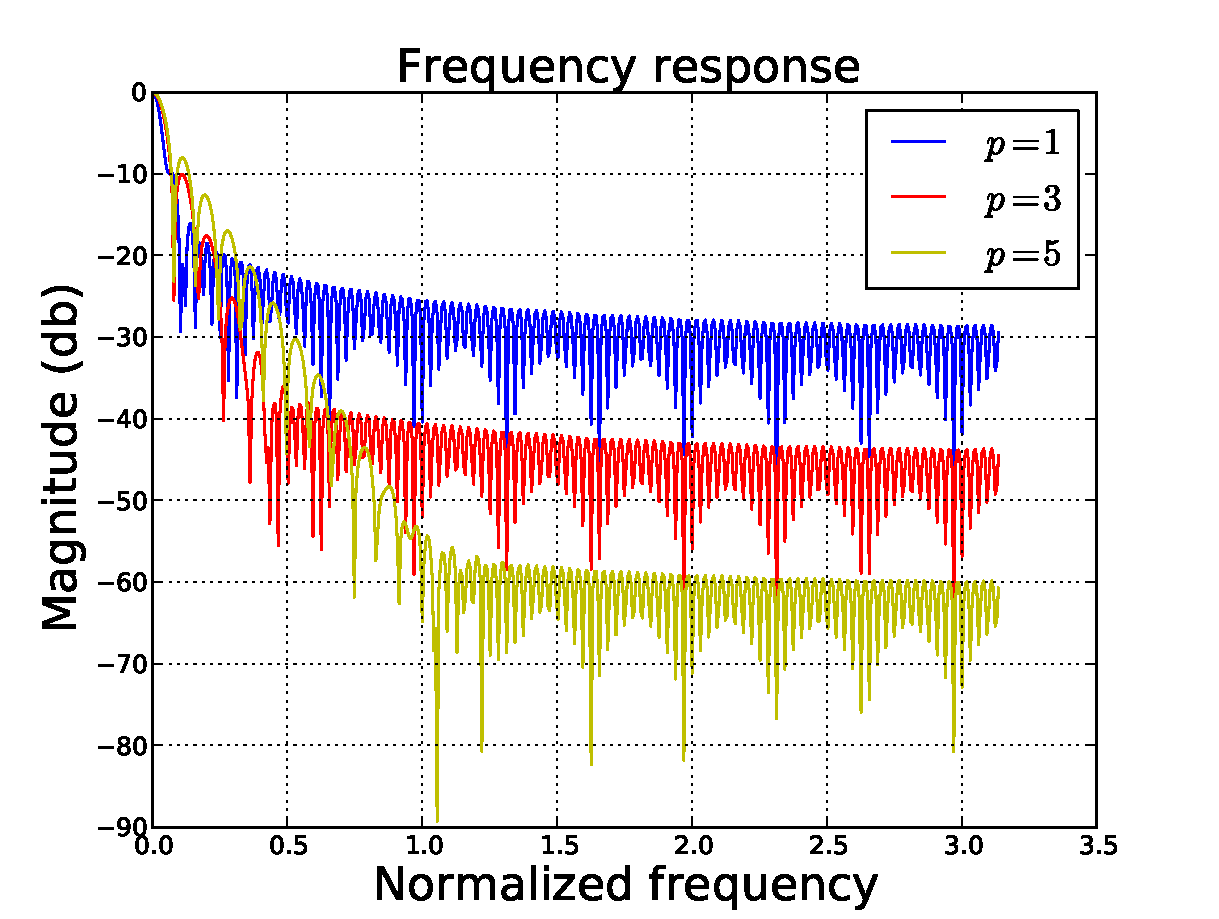
\includegraphics[width=1\textwidth]{./Figures/freq_resp_butterwordh.pdf}\caption{Overlap 
		\textit{BDWF's}: $\Delta_u t=\emptyset$.}\label{fig:fig_butter_freq}\end{minipage}\\
\begin{minipage}{0.36\linewidth}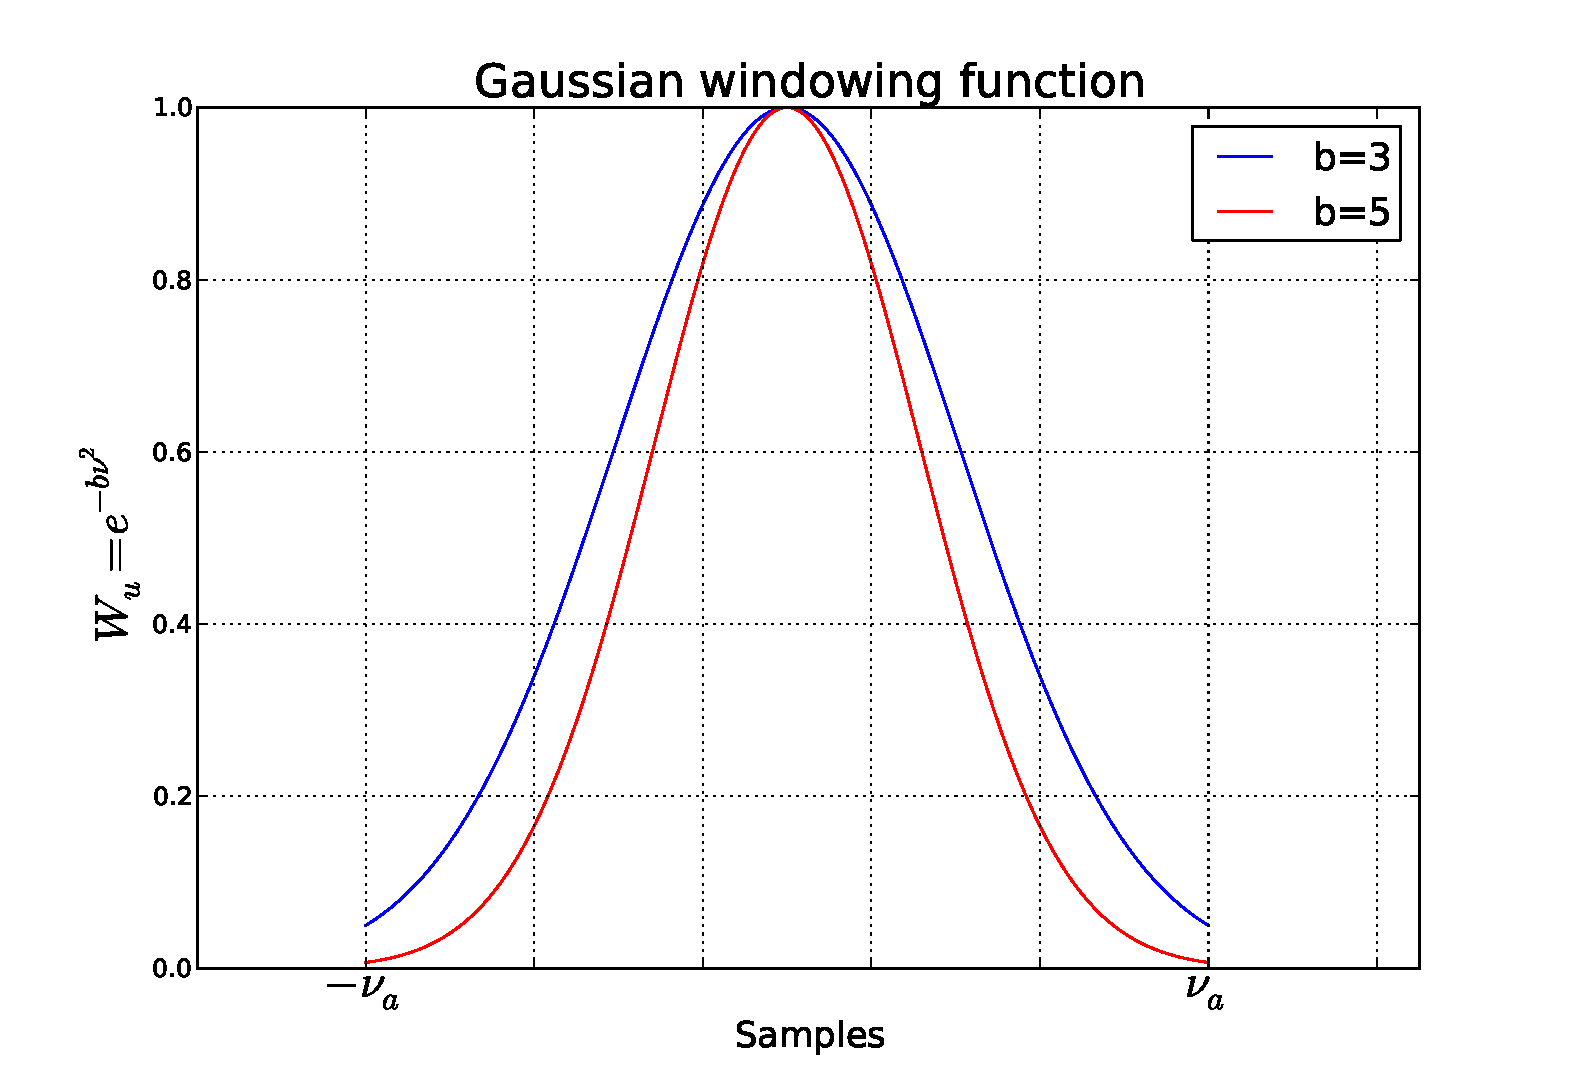
\includegraphics[width=1\textwidth]{./Figures/gausian.pdf}\caption{Overlap 
		\textit{BDWF's}: $\Delta_u t=\{250\}$.}\label{fig:fig_gauss}\end{minipage}
\begin{minipage}{0.36\linewidth}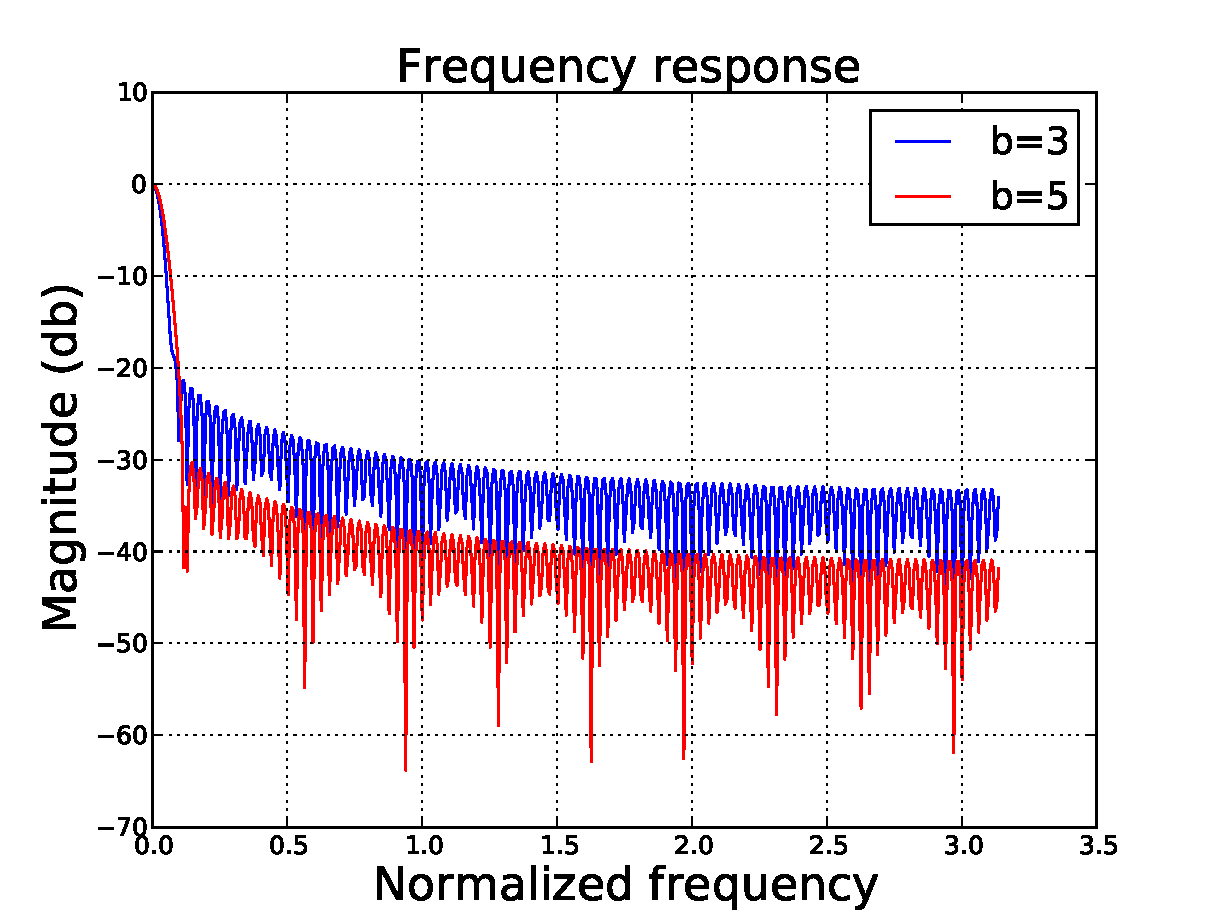
\includegraphics[width=1\textwidth]{./Figures/freq_resp_gaussian.pdf}\caption{Overlap 
		\textit{BDWF's}: $\Delta_u t=\emptyset$.}\label{fig:fig_gauss_freq}\end{minipage}
\end{figure*}
\begin{figure*}
  \centering
\begin{minipage}{0.36\linewidth}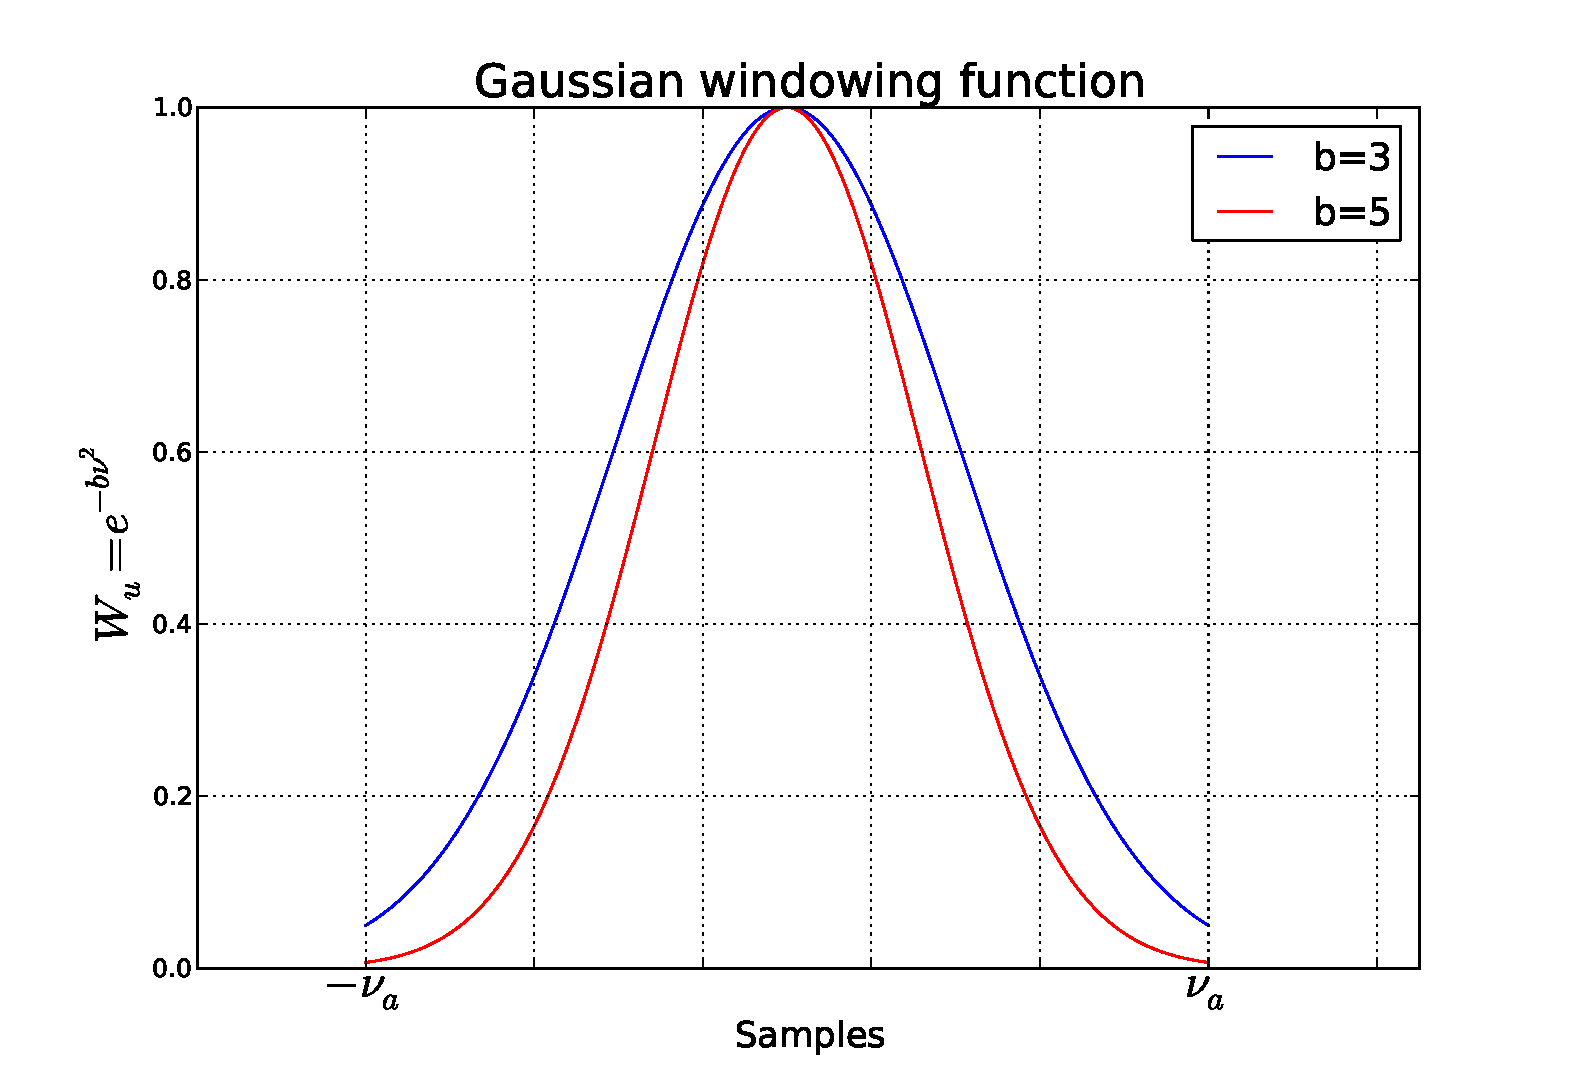
\includegraphics[width=1\textwidth]{./Figures/gausian.pdf}\caption{Overlap 
		\textit{BDWF's}: $\Delta_u t=\{250\}$.}\label{fig:fig_4}\end{minipage}
\begin{minipage}{0.36\linewidth}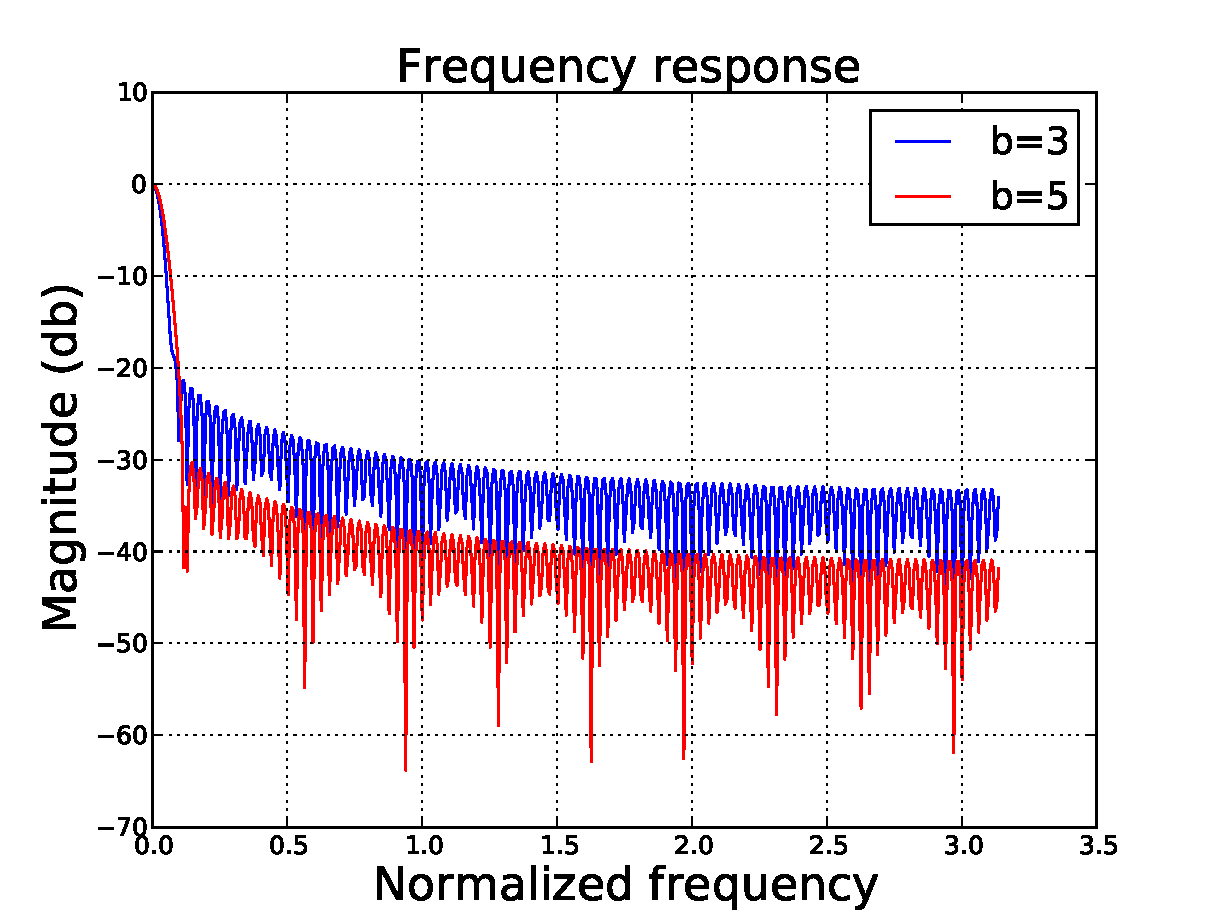
\includegraphics[width=1\textwidth]{./Figures/freq_resp_gaussian.pdf}\caption{Overlap 
		\textit{BDWF's}: $\Delta_u t=\emptyset$.}\label{fig:fig_5}\end{minipage}
\end{figure*}

$1.)$ In Figure
% The specification of the weight of the point $(u_k, v_k)$ is, $w(u_k, v_k)=e^{(\frac{-d}{s})^2}$, where $s$ measure the width 
% of the taper and $d=(u_k^2 + v_k^2)^{\frac{1}{2}}$ the baseline length.  However, the rms noise of the central pixel map is given by 
% $\sigma^2=\frac{\sum w^2(u_k, v_k)}{(\sum w^2(u_k, v_k))^2}\sigma_{obs}^2$ (see \cite{}).
% \begin{enumerate}
%  \item (Fig1a) shows the reduction of the intensity of a source at various coordinates in the sky for different $\Delta t$ with 
%        the VLA array. We measured  more than $90\%$ of the source brightness for $\Delta t \leq 25s$ when the source is within the 
%        Field of view. But, we should have compromised the large amount of data generated with shorter $\Delta t$ if the source intensity 
%        should have been drop significantly out of the field of view. For a source at coordinates (l=0, m=1deg) smearing occurs for an 
%        integration greater than 90s (see Fig1b)
%   \item (Fig1c) shows the reduction of the intensity of a source at various coordinates in the sky for different $\Delta t$ with 
%        the VLA array. We measured  more than $90\%$ of the source brightness for $\Delta t \leq 25s$ when the source is within the 
%        Field of view. But, we should have compromised the large amount of data generated with shorter $\Delta t$ if the source intensity 
%        should have been drop significantly out of the field of view. For a source at coordinates (l=0, m=1deg) smearing occurs for an 
%        integration greater than 90s (see Fig1b)
% \end{enumerate}
% \begin{enumerate}
%  \item Fig \ref{fig:fig_3a} shows three \textit{BDWF} design with a $sinc$ filter across the time direction.  
%   \item (Fig1c) shows the reduction of the intensity of a source at various coordinates in the sky for different $\Delta t$ with 
%        the VLA array. We measured  more than $90\%$ of the source brightness for $\Delta t \leq 25s$ when the source is within the 
%        Field of view. But, we should have compromised the large amount of data generated with shorter $\Delta t$ if the source intensity 
%        should have been drop significantly out of the field of view. For a source at coordinates (l=0, m=1deg) smearing occurs for an 
%        integration greater than 90s (see Fig1b)
% \end{enumerate}
\begin{figure*}
  \centering
\begin{minipage}{0.38\linewidth}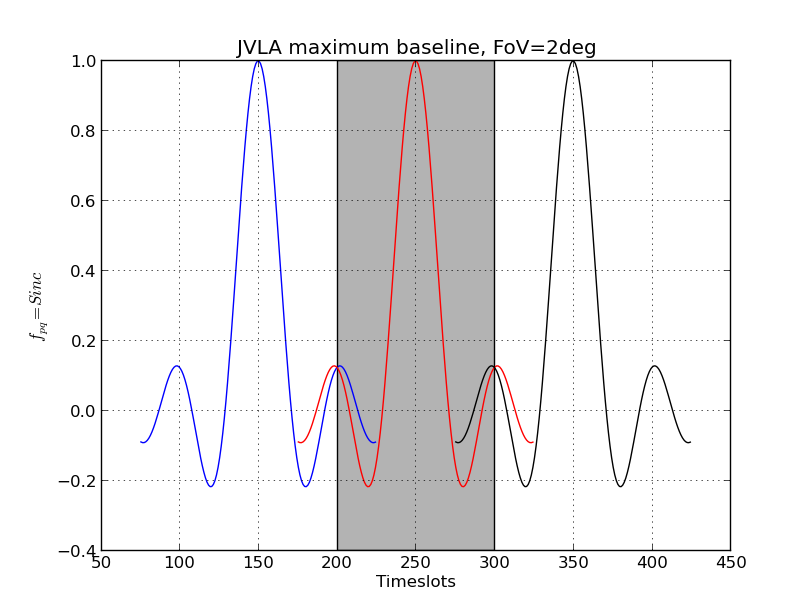
\includegraphics[width=1\textwidth]{./Figures/corrSigVLAMxBl_overlapLdelta.png}\caption{Overlap 
		\textit{BDWF's}: $\Delta_u t= [225, 250]$.}\label{ fig:fig_3a}\end{minipage}
\begin{minipage}{0.38\linewidth}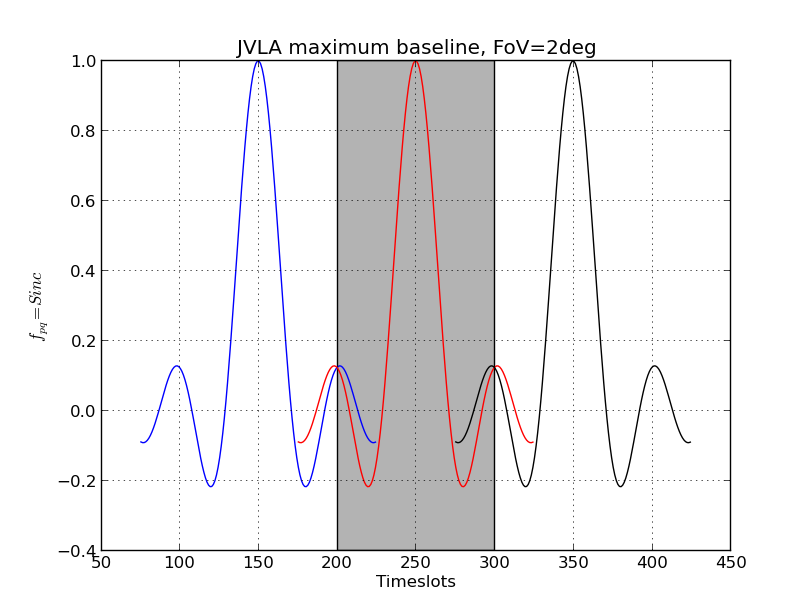
\includegraphics[width=1\textwidth]{./Figures/corrSigVLAMxBl_overlapLdelta.png}\caption{Overlap 
		\textit{BDWF's}: $\Delta_u t= [225, 250]$.}\label{ fig:fig_3a}\end{minipage}\\
\begin{minipage}{0.38\linewidth}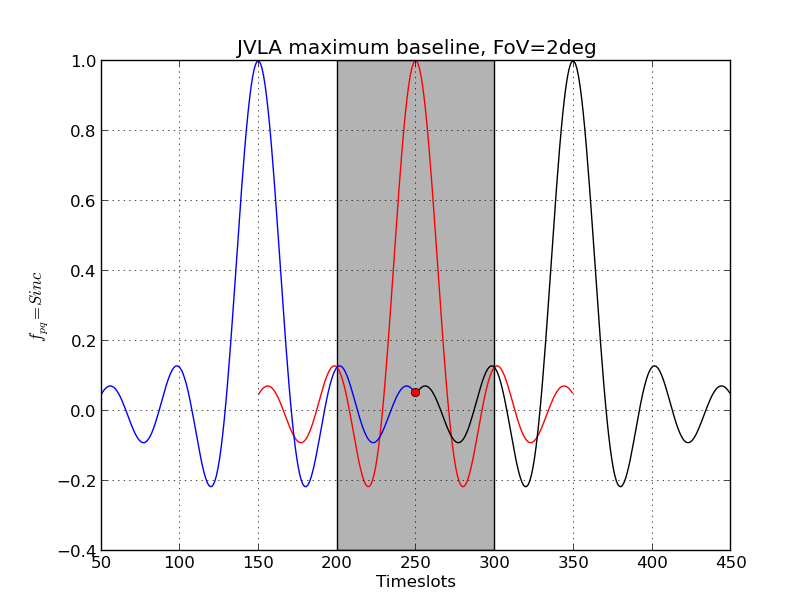
\includegraphics[width=1\textwidth]{./Figures/corrSigVLAMxBl.png}\caption{Overlap 
		\textit{BDWF's}: $\Delta_u t=\{250\}$.}\label{fig:fig_4}\end{minipage}
\begin{minipage}{0.38\linewidth}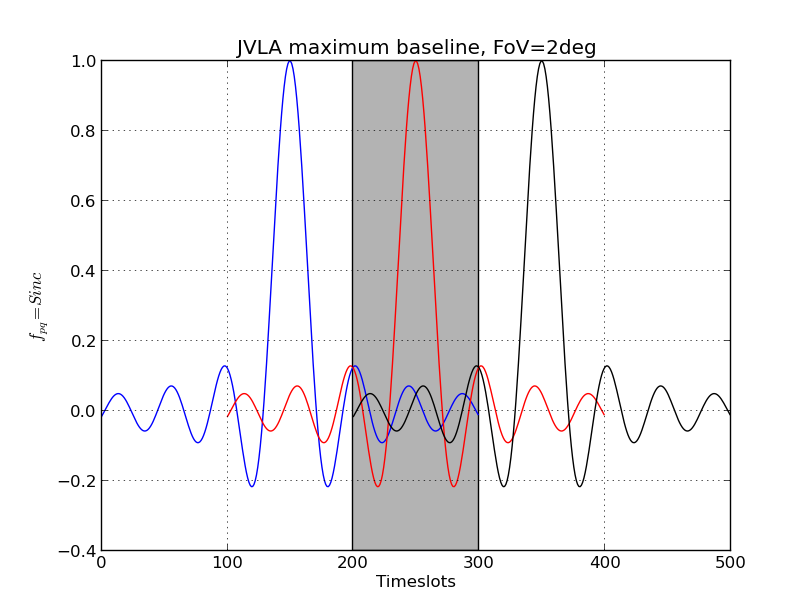
\includegraphics[width=1\textwidth]{./Figures/corrSigVLAMxBl_overlapGdelta.png}\caption{Overlap 
		\textit{BDWF's}: $\Delta_u t=\emptyset$.}\label{fig:fig_5}\end{minipage}
\end{figure*}
$1.)$ In Figures (\ref{fig1}) and (\ref{fig2}) we represented the ratio $\frac{\sigma_{meas,pq}}{\sigma_{av,pq}}$ as a function 
of $\sum_{i}^{n} u_i((t_c-t_i)/\lambda))$ ($\sigma_{meas,pq},\sigma_{av,pq}$ are the per baselines CWF and averaging rms noise  
respectively). We could also represented it as a function of baseline length. But, a uv-track corresponding to baseline aligned along the 
Est-West direction has longer tracts compare to one aligned along the South-Nordth for the same integration and frequency band. Therefore,  
$\frac{\sigma_{meas,pq}}{\sigma_{av,pq}}$ $v/s$ baselines length is ambiguous. We consider five baselines dependent 
windowing sinc function, $Bl$-$sinc$ $wk$ (with an extended width of $(k-1)n$ time intervals and/or frequency channels and $k \geq 1$). The 
experiment is done for two cases, figure (\ref{fig1}) is the one for $Bl$-$sinc$ $wk$ over both time-frequency and figure (\ref{fig2}) over 
time. These figures shows that, the noise increases with baselines length.\\

$2.)$ Figure (\ref{fig1}) shows that, with $Bl$-$sinc$ $wk$, the noise is lower on shorter baselines compared to the longer baselines. This 
is because on shorter  baselines  $\frac{\sigma_{meas,pq}}{\sigma_{av,pq}} \approx \frac{n}{n + k}$, it is the same case with 
Figure (\ref{fig2}) where $\frac{\sigma_{meas,pq}}{\sigma_{av,pq}} \approx \sqrt{\frac{n}{n + k}}$ (see the proof).  With $Bl$-$Sinc$ $wk$ 
($k>1$), the noise drops  with the extended number of time intervals and/or frequency channels of 
the window. The rate of this drop is non-linear with baselines length and also with the overlap time interval and/or frequency channels 
(see figure (\ref{fig1}b) and (\ref{fig2}b), the variation of the noise rate between baselines).  \\

$3.)$ In spite of the overlapping, with the theoretical results, the noise of longer baselines do not drop when the overlap 
samples is increased (figure \ref{fig2}). The reason is, few windows are overlapping in a visibility point when we extended in a unique 
direction (the time interval in this case) compare to two directions (time interval and frequency channels).
\begin{figure*}
 \centering
\begin{minipage}{0.38\linewidth}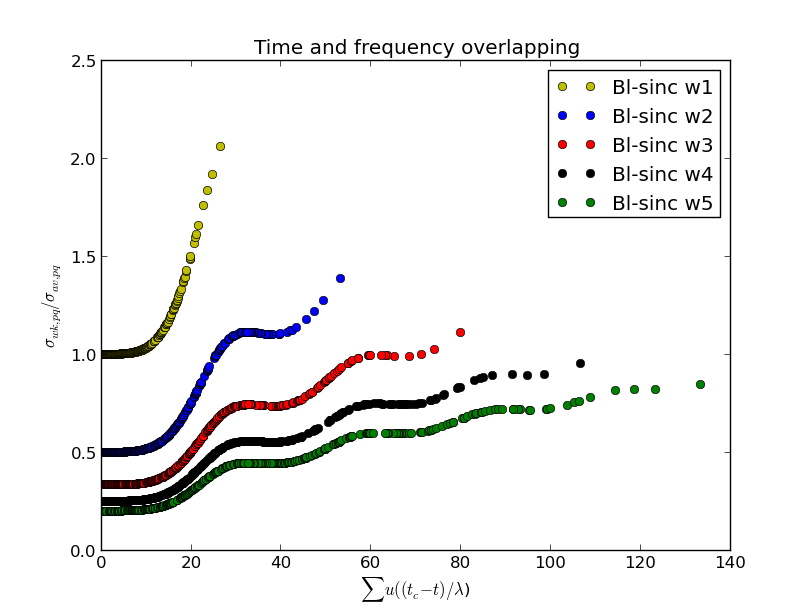
\includegraphics[width=1\textwidth]{./Figures/time_freq_ration.png}\caption{Noise ratio and rate 
of $Bl$-$sinc$-$wk$: time interval and frequency channels.}\label{ fig:fig_2a } \end{minipage}
\begin{minipage}{0.38\linewidth}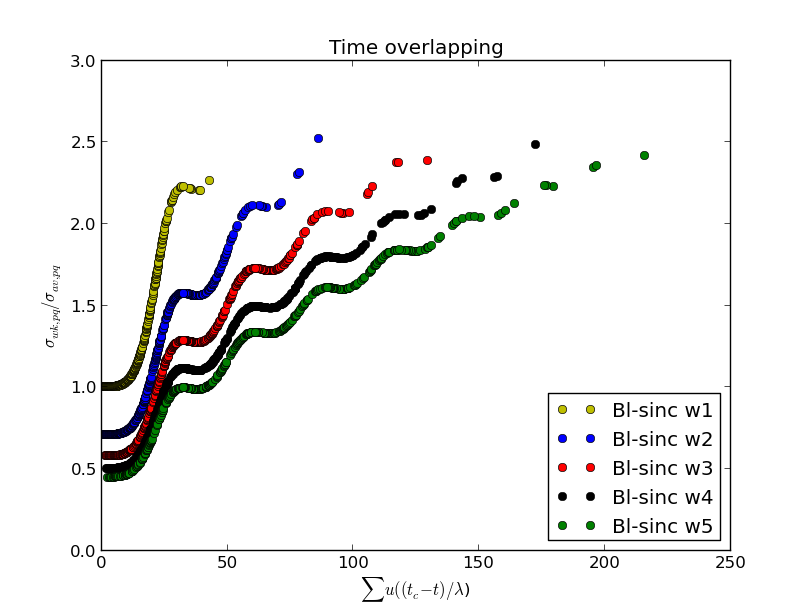
\includegraphics[width=1\textwidth]{./Figures/timeration.png}\caption{Noise ratio and rate of 
$Bl$-$sinc$-$wk$: time interval.}\label{fig:fig_2b}
\end{minipage}
\end{figure*} 
The theoretical derivation for the overall noise of $Bl$-$sinc$ $wk$ and the simulated one are quantified similarly but the pattern of the  
per baseline simulated rms noise do not look the same with the theoretical one. The number of $k$ determines the amount of noise  of CWF.
% \begin{table}
%  \begin{tabular}{|c|c|c|}
%   \textbf{Windows}&\textbf{\footnotesize theoretical analysis} &\textbf{\footnotesize simulation}\\
%   \hline\hline
%   { \footnotesize  }	  &{\footnotesize 1,066} & {\footnotesize 0,692}	\\ \cline{1-3}
% 	  
%   {\footnotesize } & {\footnotesize 1,334}& {\footnotesize 0,903} \\	\cline{1-3}
%   { \footnotesize  }	  &{\footnotesize 1,066} & {\footnotesize 0,692}	\\ \cline{1-3}
% 	  
%   {\footnotesize } & {\footnotesize 1,334}& {\footnotesize 0,903} \\	\cline{1-3}
%   { \footnotesize  }	  &{\footnotesize 1,066} & {\footnotesize 0,692}	\\ \cline{1-3}
% 	  
%   {\footnotesize } & {\footnotesize 1,334}& {\footnotesize 0,903} \\	\cline{1-3}
% \end{tabular}
% \caption{Theoretical and simulation results of the overall rms noise ratio : time interval and frequency channels.}
% \end{table}
% \pagebreak
% \begin{table}
%   \hspace{0cm}\begin{tabular}{|c|c|c|}
%   
%   \textbf{Windows}&\textbf{\footnotesize theoretical analysis} &\textbf{\footnotesize simulation}\\
%   \hline\hline
%   { \footnotesize  }	  &{\footnotesize 1,066} & {\footnotesize 0,692}	\\ \cline{1-3}
%     
%   {\footnotesize } & {\footnotesize 1,334}& {\footnotesize 0,903} \\	\cline{1-3}
%   { \footnotesize  }	  &{\footnotesize 1,066} & {\footnotesize 0,692}	\\ \cline{1-3}
% 	  
%   {\footnotesize } & {\footnotesize 1,334}& {\footnotesize 0,903} \\	\cline{1-3}
%   { \footnotesize  }	  &{\footnotesize 1,066} & {\footnotesize 0,692}	\\ \cline{1-3}
% 	  
%   {\footnotesize } & {\footnotesize 1,334}& {\footnotesize 0,903} \\	\cline{1-3}
% \end{tabular}
% \caption{Theoretical and simulation results of the overall rms noise ratio : time interval and frequency channels.}
% \end{table}
% \pagebreak
% \subsection{Analysis of $\mathcal{R}=\mathcal{F}^{-1}\{\mathcal{W}\}$}
% The CWF for each time interval  can be combined into a single two dimensional matrix,
% \begin{equation*}
% \mathcal{W}=
%   \begin{bmatrix}
%     W_{11} & W_{12} & \dots & W_{1n}\\
%     W_{21} & W_{22} & \dots & W_{2n}\\
%     \vdots & \vdots & \vdots & \vdots\\
%     W_{n1} & W_{n2} & \dots & W_{nn}\\
%   \end{bmatrix}
% \end{equation*}
\section{Simulation and results}
In order to test the algorithmics described in section and section, we performed  multiple tests on JVLA simulated measurement set 
(dataset). In this section we summarize and discussed those results.
\subsection{Data compression}

\subsubsection{Maximal integration time interval}
\subsubsection{Maximal integration frequency interval}
\subsection{Sidelobes suppression}
\subsubsection{Dataset with one strong off-axis source}
\subsubsection{Dataset with many sources}
\subsection{Discussion}
\section{Conclusions}
The goal of this paper was threefold. The first objective was to investigate **** windowing functions***\\
The second objective  was to study ****first algorithm data compression***\\
The final objective was to ****second algorithm data compression and out field suppression*** \\
Drawback and futures works*** drawback and futures works*****

\section*{Acknowledgements}
\bibliographystyle{mn2e}
\bibliography{m_paper}
\appendix
\section[]{Demonstration}
The proof of the norm used in Section~\ref{sec:t_der} is given below.\\
if $||\textbf{U}_{pq,t}||_{m}=\Bigg(||\mathbf{u}_{pq,t_s}||, \dots , ||\mathbf{u}_{pq,t_c}||, \dots, ||\mathbf{u}_{pq,t_e}||\Bigg)$ is a 
$n_t\times2$ matrix, where each element $||\mathbf{u}_{pq,t_i}||$ is a vector of size 2 and $||.||$ is an Euclidean norm, then $||.||_{m}$ 
is a norm.
\begin{proof}
\begin{enumerate}
 \item $||\mathbf{U}_{pq,t}||_{m}\geq \mathcal{O}_{E}$
 \item $||\mathbf{U}_{pq,t}+\mathbf{U}_{pq,t}'||_{m} \leq ||\mathbf{U}_{pq,t}||_{m} + ||\mathbf{U}_{pq,t}'||_{m}$
\end{enumerate}
\end{proof}
\bsp
\label{lastpage}
\end{document}
